\documentclass[12pt]{article}

\usepackage[top=0.75in,bottom=0.75in,left=0.75in,right=0.75in]{geometry}
\usepackage{amsmath,amssymb,multirow,graphicx}

% Comments for making sure we touch all the bases for a good paper
\newif\ifcommentsw
\commentswtrue
\newcommand{\comment}[1]{\ifcommentsw  $\blacktriangleright$\ \textbf{#1}\ $\blacktriangleleft$ \fi}
%\commentswfalse   % remove the % to turn off informational comments 


% Notes on the paper for communicating with coauthors
\newif\ifnotesw
\noteswtrue
\newcommand{\notes}[1]{\ifnotesw  $\bullet$\ \textit{ \textbf{#1}}\ $\bullet$ \fi}
%\noteswfalse   % remove the % to turn off notes to coauthors


\newcommand{\br}{\mathbf{r}}
\newcommand{\sgn}{\operatorname{sgn}}
\def\cq{{\emph{Culex quinquefasciatus} }}

\title{Agent-based simulations of mosquito-host encounter rates}
\author{
\textbf{Ricardo Cortez}\\
   \small{Mathematics Department}\\
   \small{Tulane University}\\ \and
\textbf{Bree Cummins}\\
   \small{Mathematics Department}\\
   \small{Tulane University}\\ \and
\textbf{Ivo M. Foppa}\\
   \small{Department of Epidemiology}\\
   \small{Tulane University}\\ \and
\textbf{Justin Walbeck}\\
   \small{Mathematics Department}\\
   \small{Tulane University}\\ 
}


\begin{document}
	
	\tableofcontents
	
	\maketitle
	
\section{Introduction}
Transmission of many infectious agents is ``heterogenous'', which means that the risk for infection and infectiousness are unevenly distributed over the population \cite{Woolhouse1997}.
If heterogeneity is ignored in transmission models, misleading inference about transmission dynamics might result: Typically, the ability of an infectious agent to persists will be underestimated \cite{Hasibeder1988}.
One source of heterogeneity in mosquito--borne disease transmission is uneven distribution of mosquito bites over hosts \cite{Dye1986}.
The number of mosquito that bite an individual host receives must depend on  the number of mosquitoes that find that host.
Host finding of mosquitoes is largely driven by olfactory cues that are given off by individual hosts \cite{Lehane1991}.
We might therefore expect that  the way  feeding hosts of mosquitoes are spatially arranged will affect the mosquitoes' probability of success in locating and feeding on them. Most vertebrate hosts are spatially aggregated.
Unless that the probability of finding a host is exactly proportional to the local density of hosts,
unevenly distributed biting rates on individual hosts and thus heterogenous disease transmission will result.

The work presented here was originally motivated by the observation that birds that some species of birds that are particularly vulnerable to West Nile virus infection, in particular the American crow (\textit{Corvus brachyrhynchos}) tend to congregate in large roosts. These birds often suffer catastrophic mortality during West Nile virus epizootics. The question therefore arose how the roosting behavior of birds and catastrophic changes in roost structure may affect the transmission dynamics of this mosquito--borne virus.

Answering this question requires a detailed understanding of how the spatial arrangement of hosts will affect the distribution of mosquito bites on these hosts.

The difficulties of approaching this question experimentally makes
Agent-based simulations a natural way to exploring this problem under a range of assumptions about host and  mosquito behavior and odor dispersal.
Here, we specifically seek to explore the effect of host aggregation on a small-scale spatial on the per--capita biting rate.

We first give an overview of relevant mosquito behaviors, by reviewing what is known about the different stages of the appetitive flight of mosquitoes. 
We then ...

\section{Overview of mosquito host-seeking behavior}\label{sec:mosqbehav}

The diurnal cycle triggers host-seeking behavior in mated female mosquitoes. Typically this behavior begins when the mosquitoes are very far from the hosts, and ends after a successful bite. We are interested in the intermediate spatial scale of host-seeking behavior, when the mosquitoes are tens of meters to tens of centimeters from a host. On this scale, it is useful to classify the host-seeking behavior in terms of two functional regimes that we will call ranging flight (flight without an odor cue) and homing flight (flight in the presence of an odor cue). Homing flight has been carefully studied in laboratory and field wind tunnel experiments, but ranging flight is not well-characterized.

\subsection{Homing flight}

Odor cues are complex olfactory signals released from a host's skin and breath. There are many chemicals known to excite the chemoreceptors of mosquitoes, for example CO$_2$, lactic acid, and various aldehydes \cite{Bowen1991,Syed2009}. CO$_2$ is a very important component in the odor plume that activates and helps maintain homing flight \cite{Bowen1991,Gibson1999,Gillies1980}. Activation thresholds for the mosquitoes \emph{Aedes aegypti} and \emph{Anopheles gambiae} are 1000-3000 ppm \cite{Gibson1999}. Mosquitoes are sensitive to changes in CO$_2$ concentration as small as 100 ppm \cite{Gillies1980}.

In the absence of wind, chemical signals are dispersed primarily by diffusion. In the presence of uniform, laminar wind, the host odor extends into a long, thin plume with sharp transverse gradients and shallow longitudinal gradients. If the wind is turbulent, then the plume is characterized by a high degree of intermittency, but it still retains relatively shallow average longitudinal gradients compared to the transverse gradients \cite{Vickers2000}. 

Odor plume structure is important to mosquito behavior. Gillies \cite{Gillies1980} reports that sustained flight in laboratory wind tunnels only occurs in the presence of an intermittent CO$_2$ signal and not in uniform concentrations. Dekker et al. \cite{Dekker2005,Dekker2001} similarly find that broad, well-mixed CO$_2$ plumes inhibit upwind flight, while turbulent plumes of the same concentration induce upwind flight in a laboratory wind tunnel.

Mosquitoes must be able to locate hosts both in windy and windless conditions. In the absence of wind, mosquitoes must rely solely on odorant cues \cite{Vickers2000} or on large features in the visual environment \cite{Bidlingmayer1994}. If an odorant signal is present, it is probable that mosquitoes sample the odorant over time to estimate the gradient, as tsetse flies seem to do \cite{Carde1996}. 

When there is wind present, it provides additional information to the insect, since any odorant source presumably originates upwind. Wind speeds of interest are usually 1 m/s or less, since mosquitoes cannot fly much faster than this on a sustained basis \cite{Clements1999}. Mosquitoes use vision to estimate the wind direction by watching the optical flow of ground features \cite{Carde1996}. In the presence of an odor cue, mosquitoes travel upwind in an attempt to locate the source in both laboratory and field wind tunnel experiments \cite{Cooperband2006, Dekker2005,Dekker2001}. Many organisms have characteristic turns in their upwind flight path (e.g. moths, \cite{Carde1996,Vickers2000}), but mosquitoes and tsetse flies exhibit highly irregular upwind flight, possibly to confound host defensive behaviors \cite{Davis1996}.

\subsection{Ranging flight}

Unlike homing flight, ranging flight behavior remains mostly uncharacterized. If wind is absent, orientation may be determined by large visual features in the environment \cite{Bidlingmayer1994}, or may be best characterized as an unbiased random walk. If wind is present, then the mosquitoes may deliberately choose to fly upwind, downwind, or crosswind in search of a host. Each of these three behaviors is plausible based on either experimental or theoretical work. Gibson and Torr \cite{Gibson1999} report that mosquitoes typically fly upwind in wind tunnels even when there is no odorant present. Gillies and Wilkes \cite{Gillies1974} conducted a set of field experiments that provided evidence for downwind flights in host-seeking \emph{Mansonia} mosquitoes. Dusenbery \cite{Dusenbery1989} argued that crosswind searching is mathematically optimal when the odor plumes are long and thin. Sabelis and Schippers  \cite{Sabelis1984} agree with that result when the variability of the wind direction is less than 30 degrees from the mean. If greater than 30 degrees, they argue that either upwind or downwind searching is mathematically optimal. 

Our goal is to develop a general model that can account for these different host-seeking behaviors and assess their impact on the number of mosquito-host encounters in a given scenario. 

\section{Numerical model}
	
	\comment{Bree: Add table of mathematical symbols. Maybe caps for dimensional functions, lowercase for nondimensional?}

	We describe a coupled PDE/agent-based model that simulates the behavior of mosquitoes interacting with an odor plume. Although we have made particular choices about the structure of the simulated odor plume and the behavior of the agents representing the mosquitoes, these algorithms are modular and flexible, so that different physical and biological scenarios may be easily fit into this modeling framework. 
	
	The model can be described in terms of three components: (1) the evolution of a concentration plume used by the mosquitoes to seek out hosts, (2) the behavior of the mosquitoes, and (3)  the behavior of the hosts.  The transmission dynamics is assumed to occur in a two-dimensional rectangular region whose sides are of length $L_x$ and $L_y$. A population of $N_v$ mosquitoes (e.g. {\sl Cx. quinquefasciatus}) are given independent entrance times and entrance locations into the domain. Initial populations of $N_h$ hosts (e.g. birds) are placed in several subregions of the domain.
	
	
	\subsection{Simulated odor plumes}
 	The first component of a transmission dynamics model is the mosquito-host
		interaction, including the mechanisms that mosquitoes use to find hosts.  Our model is based on
		the assertion that hosts release a fixed amount of CO$_2$ (or some other gaseous clues) per host per
		unit time.  This concentration plume is then diffused and possibly convected by wind within the
		two-dimensional region. The convection velocity of the wind is assumed to be represented by
		the known divergence-free velocity vector ${\vec U}(x,y,t)$.  The concentration $C(x,y,t)$ satisfies the
		advection-diffusion equation
		\begin{equation}\label{eq:conv-diff}
		\frac{\partial C}{\partial t} + ({\vec U + \vec U_r})\cdot\nabla C = D\nabla^2 C + S(x,y),
		\end{equation}
		where $t$ is time, and $(x,y)$ are spatial coordinates.  $D$ is the (constant) diffusion coefficient
		and can be adjusted to reflect the speed at which the particular substance of interest diffuses in air.
		The transport velocity ${\vec U}$ can be used to introduced drifts or relatively large features
		produced by the air. We add a random velocity vector $\vec U_r$ with zero mean to approximate the effect of small-scale turbulence in the domain. \comment{Bree: Might want to reformulate in conservation form.} The last term
		represents the source of CO$_2$ concentration at the host locations. In our model, we will consider
		this term to be $S(x,y) = S_0 \sum \delta(x-x_h,y-y_h)$ where $S_0$ is a constant concentration emission per
		unit time and the delta function reflects the fact that the CO$_2$ occurs only at the host locations.
		
		Although Eq.~(\ref{eq:conv-diff}) is continuous in space and time, to simulate this spread
		computationally, we use a discrete grid of spacing $h$ that covers the two-dimensional
		domain $\Omega = L_x \times L_y$. We use $x_j = jh$ and $y_k = kh$ (with $h N_x = L_x$ and $h N_y = L_y$).
		Then $C^n_{j,k}$ approximates $C(x_j,y_k,t_n)$ and its second derivatives are approximated
		using center-differences
		\[
		\frac{\partial^2 C}{\partial y^2}(x_j,y_k,t_n) \approx \frac{ C^n_{j,k+1} - 2C^n_{j,k} + C^n_{j,k-1} }{h^2}
		\hskip20pt etc.
		\]
		The advection terms are calculated using an upwinding scheme:
		\[
		u\frac{\partial C}{\partial x}(x_j,y_k,t_n) \approx \max({u,0})\frac{C^n_{j,k} - C^n_{j-1,k}}{h} + \min({u,0})\frac{C^n_{j+1,k} - C^n_{j,k}}{h}
		\hskip20pt etc.,
		\]	
		where $u$ is the $x$-component of $\vec V = \vec U + \vec U_r$. We assume that the normal components of the concentration gradient are zero at the boundary (Neumann conditions for the Laplacian). \comment{Bree: We actually have outflow conditions -- might want to explain a little more rigorously.} The CO$_2$ concentration is solved for at discrete time steps of $\Delta t$. 
		
	\subsection{Host behavioral heuristics}
	Our motivating problem is the encounter rate between \cq mosquitoes and birds. Since \cq is a nocturnal species, the principal opportunities for host-mosquito interaction are during roosting periods in which the birds are relatively stationary. For this reason, the agents representing bird hosts do not move from their initial positions; however, a random walk or biased random walk could be easily introduced. Host locations are not restricted to the CO$_2$ grid.

	\subsection{Mosquito behavioral heuristics}\label{sec:rules}
	Mosquitoes are assumed to have two distinct behavioral regimes: ranging flight that occurs before a CO$_2$ signal is detected and homing flight that occurs in the presence of CO$_2$. Below a CO$_2$ threshold set by the user, $C < C_0$, the mosquitoes navigate only using wind direction and move either upwind, downwind, or crosswind. Above the CO$_2$ threshold, the mosquitoes respond by moving both upwind and up-gradient using CO$_2$ cues. Mosquito motion is not restricted to the CO$_2$ grid, and the mosquitoes may even leave and re-enter the domain. When a mosquito comes within a user-defined radius of a host, the mosquito is removed from the simulation and a ``contact" is recorded. In this context, a contact means an attempted landing or bite, not necessarily successful. 
	
	Along with a minimum sensory threshold, we assume that the mosquitoes have a saturation response to CO$_2$. Above a threshold that we call $C_{sat}$, a mosquito can no longer distinguish between different CO$_2$ concentrations. In fact, we assume that an agent responds to a generic sensory input $B(x,y,t)$ via a trigger threshold $B_0$ and a saturation level $B_{sat}$. We nondimensionalize by the saturation level: $b(x,y,t)=B(x,y,t)/B_{sat}$ and $b_0 = B_0/B_{sat}$. The shape of the agent response may then be described by the general function $F(b(x,y,t), b_0; \kappa)$:
	\begin{equation}
		F(b(x,y,t), b_0; \kappa) = \left\{ \begin{array}{lr} 0, & b < b_0 \\ \dfrac{(1+\kappa b_0)(b-b_0)}{(1+\kappa b_0 b)(1 - b_0)}, & b_0 \leq b \leq 1 \\ 1, & 1 < b  \end{array}\right. , \label{eqn:functional}
	\end{equation}
where the parameter $\kappa \in (-1/b_0,\infty)$ controls the concavity of the response function (see Figure~\ref{fig:exampleF} for examples). 

\begin{figure}[htp]
\begin{tabular}{ccc}
	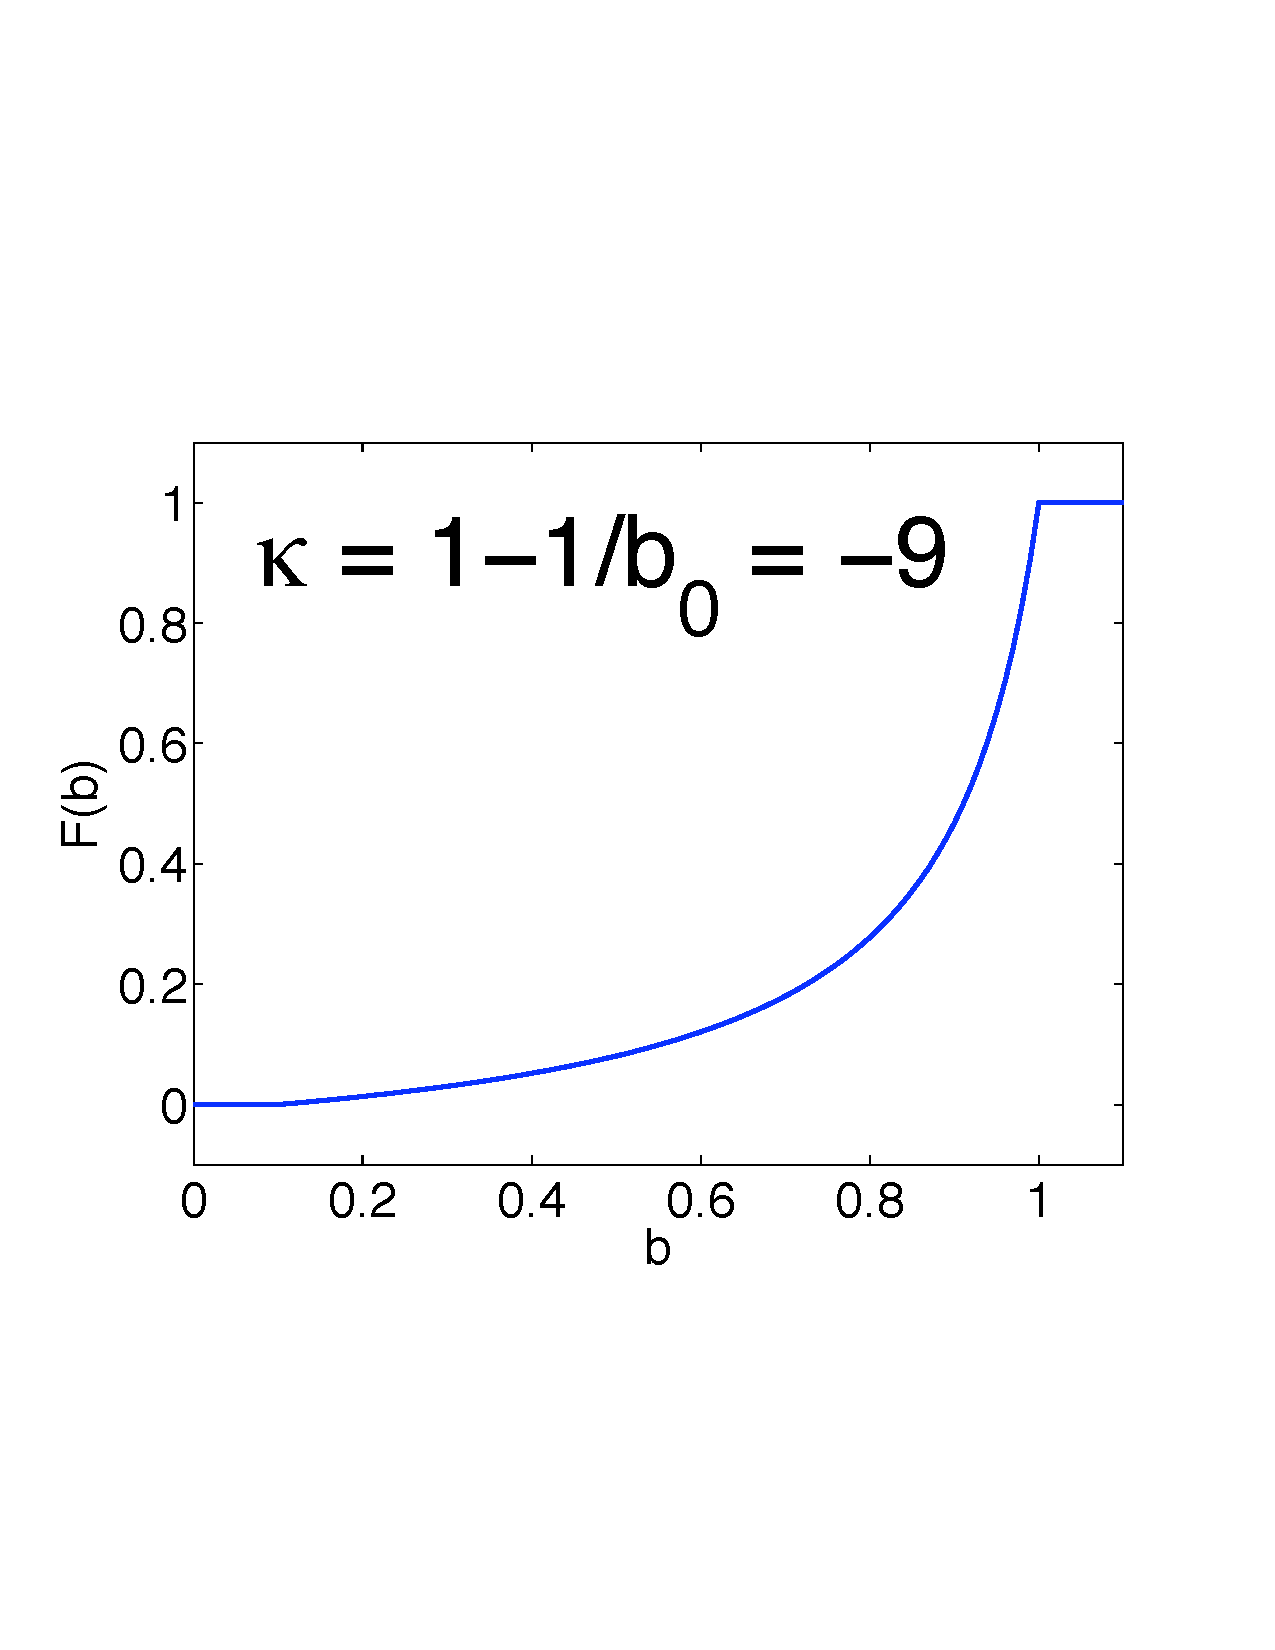
\includegraphics[width=2.25in]{figures/Fconcaveup.pdf} & 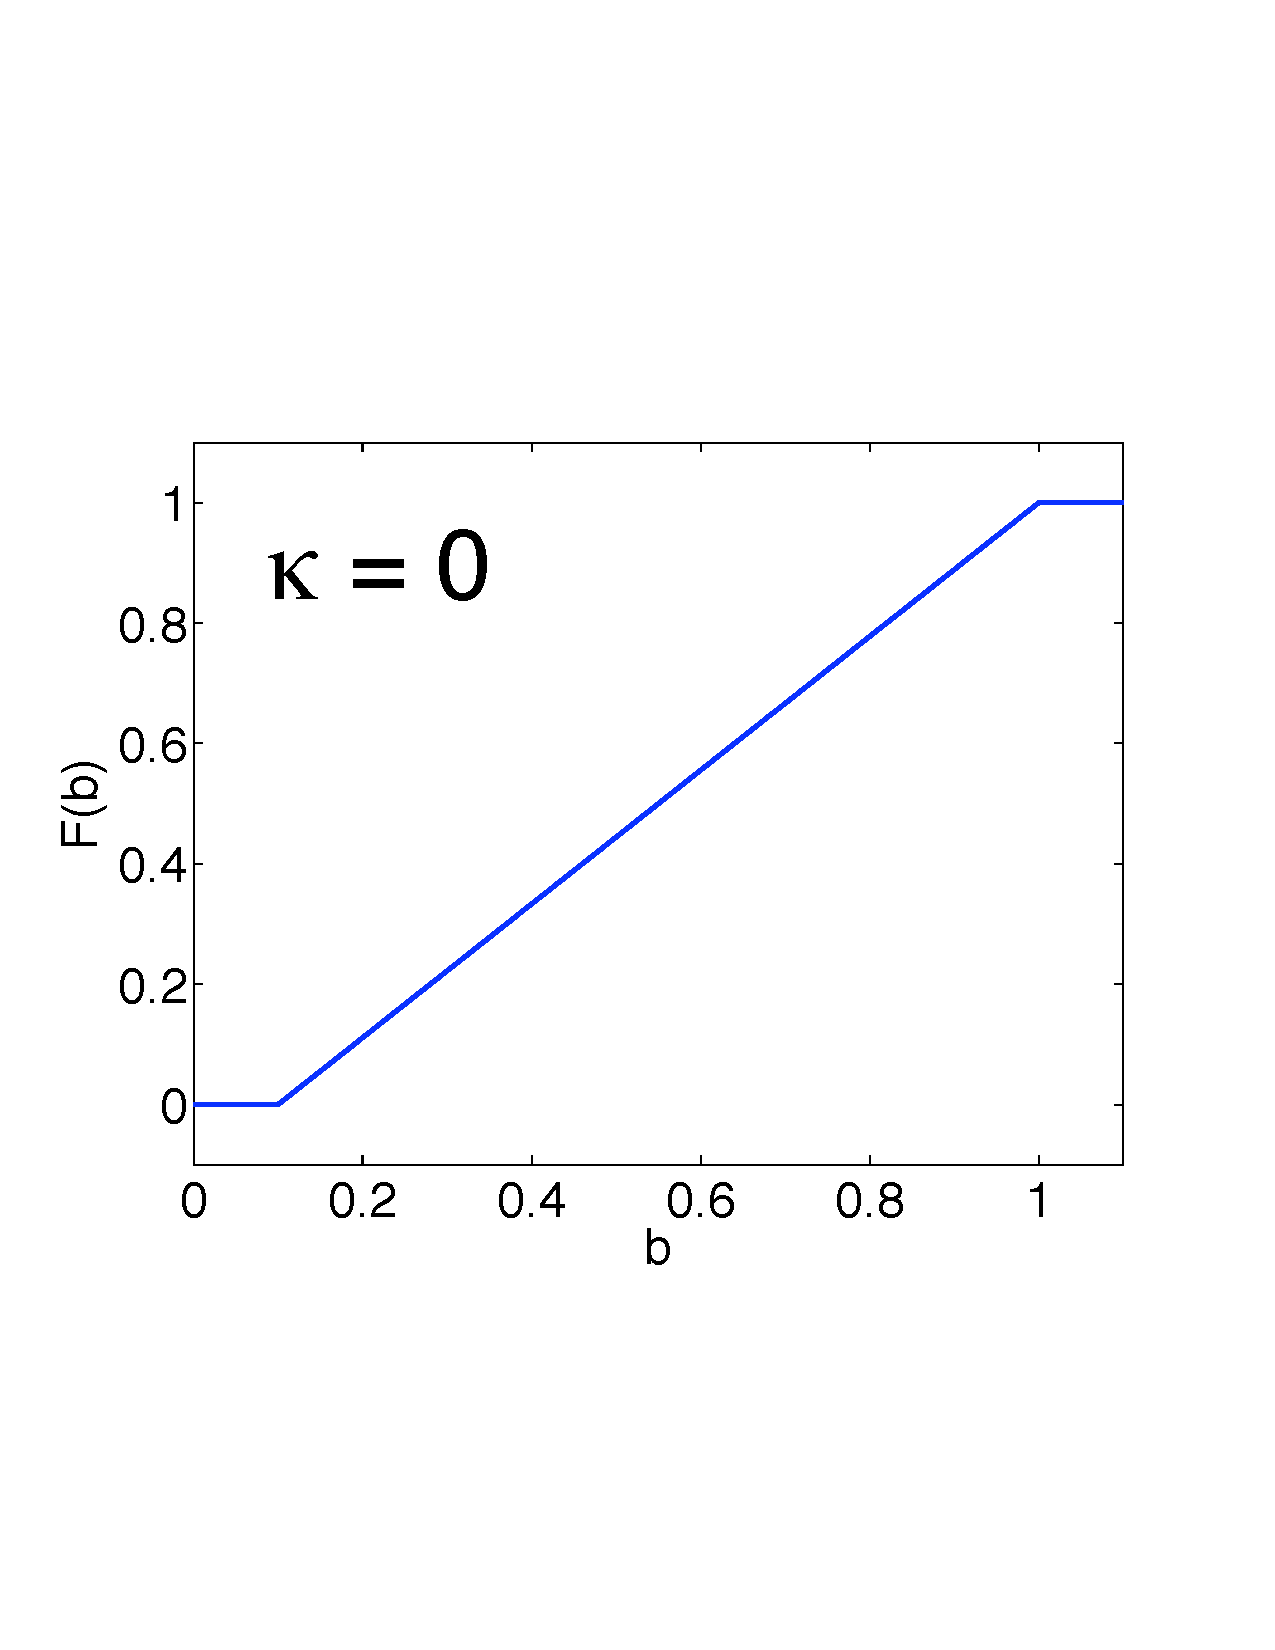
\includegraphics[width=2.25in]{figures/Flinear.pdf} & 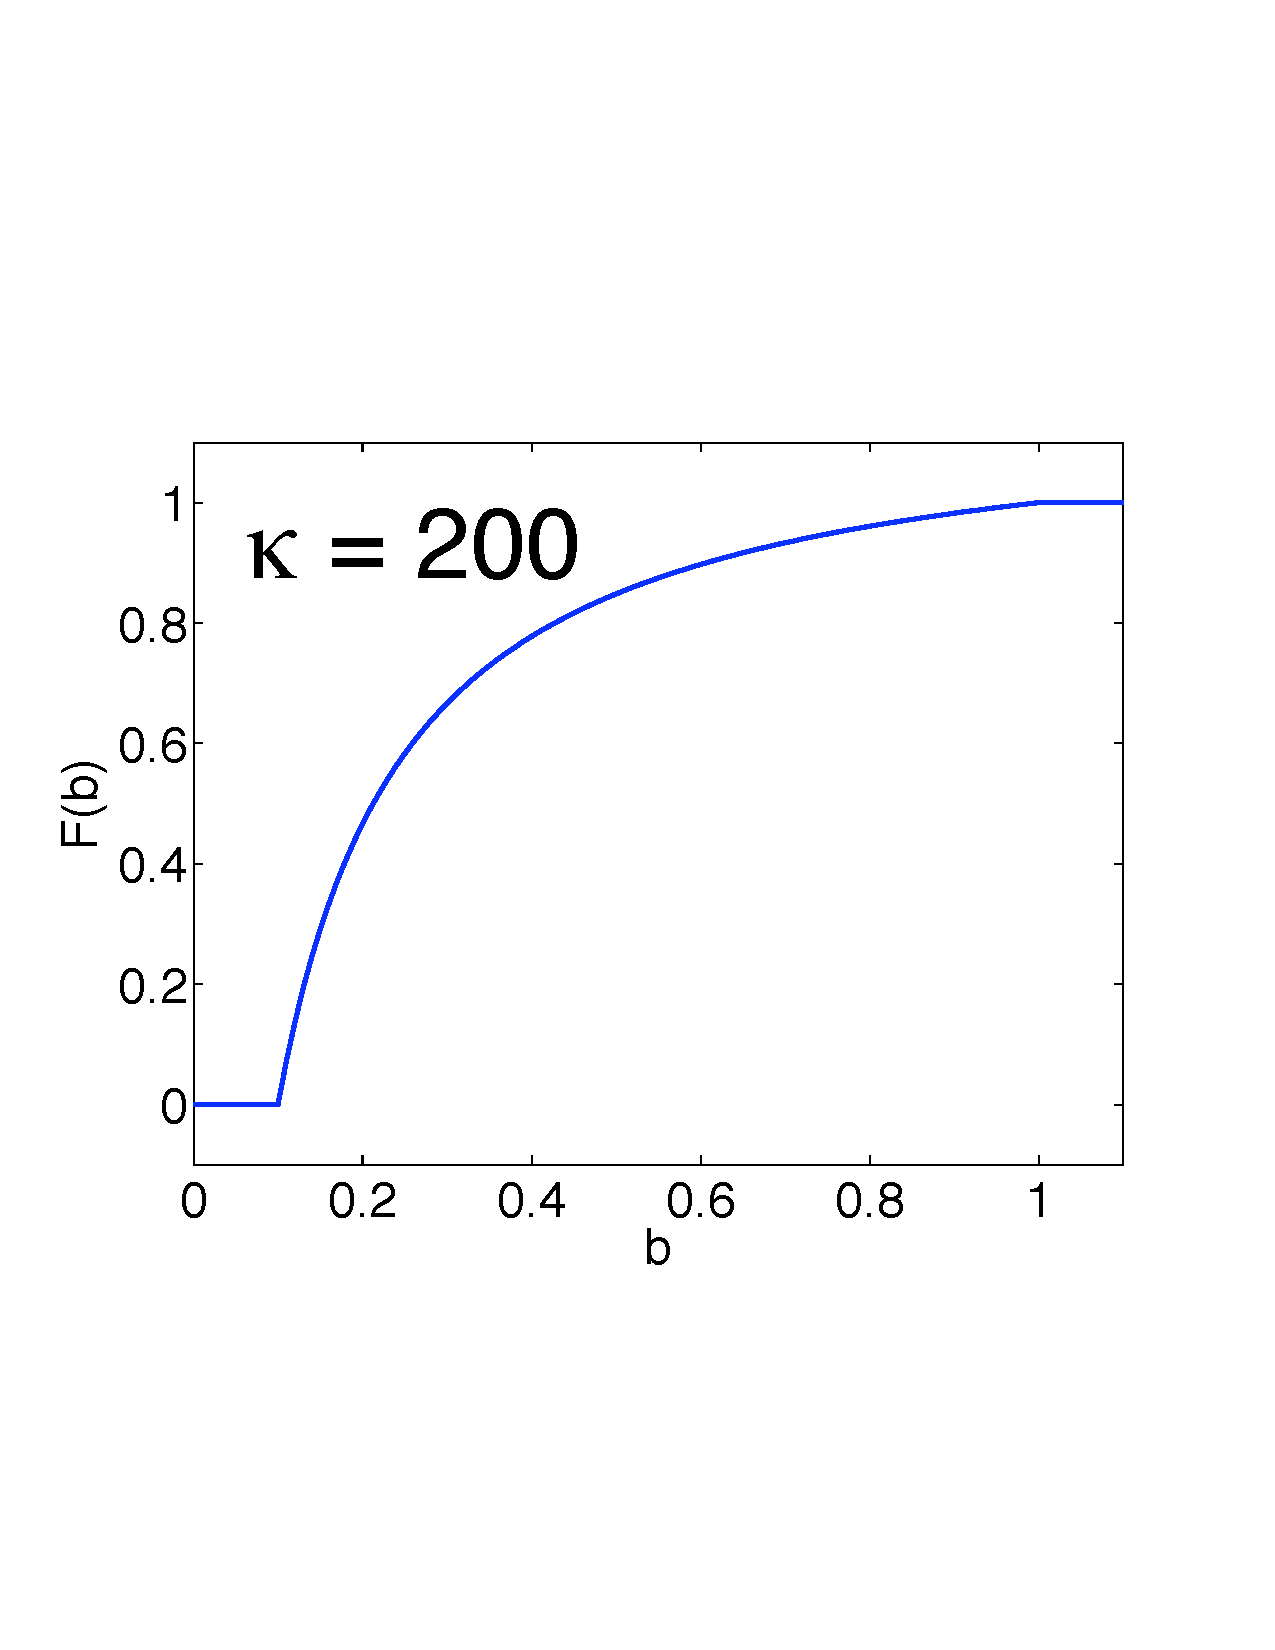
\includegraphics[width=2.25in]{figures/Fconcavedown.pdf}
\end{tabular}
\caption{The parameter $\kappa$ controls whether the response of the agent is concave up or down with respect to the sensory input. For these figures, $b_0 = 0.1$.}
\label{fig:exampleF}
\end{figure}

	
	We assume that mosquito agent decisions are all numeric values that fall within a range $[p_1, p_2]$ with exact values $p$ determined by the response to a sensory input $b(x,y,t)$:
	\begin{equation}
	p  = p_2 - (p_2 - p_1)F(b(x,y,t), b_0; \kappa). \label{eqn:response}
\end{equation}
	This equation ensures that $p$ takes on the highest values when the sensory input is lowest. In the remainder of this section, we describe several aspects of agent behavior that are determined by Eq.~\eqref{eqn:response}.
	

	\subsubsection{Response to wind}
	
	As mentioned in Section~\ref{sec:mosqbehav}, there is a relatively strong consensus that mosquitoes, even nocturnal fliers, use optical flow to estimate their relative heading with respect to wind direction. Simulating this mechanism in our model would add substantial complexity, since it would require calculating drift over a reference ground pattern that is governed by a set of free parameters. Instead, we choose to model the wind sensing capability of the mosquitoes as a ``precision window'' around the direction of the wind, where the stochasticity of the agent response is intended to mimic the average behavior that would occur over many possible ground patterns. It is then straightforward to calculate the wind direction from interpolated wind vectors at the nearest grid points, and to choose a random direction within the precision window. During ranging flight, we assume that the mosquitoes fly at constant speed greater than the mean wind speed, so that upwind flight is possible. 
	
	Let $\theta_v$ be the direction of the wind $\vec V$ at $(x,y)$ and time $t$. When $C < C_0$, the mosquitoes are exhibiting ranging flight behavior and their target directions, $\theta_v + \psi$, depend on their assigned flight strategy: $\psi=0$ for downwind flight, $\psi=\pi$ for upwind flight, and $\psi \in [-\pi/2, -\pi/4] \cup [\pi/4,\pi/2]$ for varying degrees of crosswind flight. We model the mosquito's precision window by $\pm\alpha$, where $\alpha$ is given by 
	\begin{equation}\label{eqn:alpha}
	\alpha = \alpha_2 - (\alpha_2 - \alpha_1)F(\vec V(x,y,t), V_0; \kappa).
\end{equation}
	In the above equation, $\alpha_1$ and $\alpha_2$ denote the smallest and largest amounts of imprecision in the mosquito's estimate of wind direction. We assume that saturation occurs at $\max |\vec V|$ \comment{Bree: May want some other value.}, that the sensory threshold $V_0$ is 0, and that $\kappa = 0$.
	
	The mosquito's final direction of motion is given by
	\begin{equation}\label{eqn:thetav}
	\Theta_v =  \left\{\begin{matrix}\theta_v + \psi + \eta\alpha, & C < C_0, & \text{$\psi$ varies with wind strategy} \\  \theta_v + \pi + \eta\alpha, & C \geq C_0, & \text{upwind strategy,} \qquad \qquad \: \: \: \end{matrix} \right. 
\end{equation}
	where $\eta$ is a uniformly distributed random variable in $[-1,1]$. The above equation includes the case where $C \geq C_0$ and the mosquito is engaged in homing flight. However, only part of the mosquito motion is determined by the upwind strategy when $C \geq C_0$. The other part is determined by the CO$_2$ concentration.
	
	
	\subsubsection{Response to CO$_2$: Exploration of chemotaxis rules}\label{sec:chemostats}
	
	There are many possibilities for modeling positive chemotaxis that do not substantially increase the complexity of our model. A simulated mosquito agent may sense the absolute amount of CO$_2$ or its gradients, and may adjust its heading, speed, or both in response. In this section we present a comparison between different chemotactic heuristics, any of which may be easily substituted into the model framework. 
	
	\textbf{Problem specification:} To more easily evaluate the heuristics, we consider a simplified problem with a steady state CO$_2$ gradient. An odorant point source is located at $(0.4L,0.3L)$ in a box that is $L$ units on a side. The source decays exponentially as $C(r) = e^{-40r^2}$, where $r$ is Euclidean distance from the source. Two hundred mosquitoes are randomly distributed in the area $(0.75L,0.85L)$ by $(0.75L,0.85L)$ at time $t=0$. These mosquitoes do not interact with each other (they may superpose in space) and they do not affect the chemical distribution. We nondimensionalize the problem using a typical mosquito speed $s_0$ and the domain length $L$. We take $s_0 = 1$ m/s and $L \approx 20$ to $30$ m. Mosquitoes make navigation decisions every $\Delta t = 0.01L/s_0 \approx 0.2$ to $0.3$ s. The mosquitoes are prevented from leaving the domain. 
	
	\textbf{Chemotactic heuristics:} We first discuss mosquito heading. In order to choose a flight direction, a mosquito can either estimate the CO$_2$ spatial gradient and travel up the gradient, or it can compare the CO$_2$ levels at previous locations to assess the goodness of its current heading. Both of these strategies would require physical structures on the mosquito: the first requires that CO$_2$ sensors be sufficiently dispersed across the body in order to estimate the spatial gradient and the second requires the mosquito to have a memory. In terms of mosquito biology, the first requirement may not be fulfilled, since the known CO$_2$ sensors are located on small appendages called palps clustered near the mouthparts~\cite{Bowen1991}. But computationally speaking, it is more convenient to use the spatial gradient than to provide agents with a memory. 
	
	We explore both of these behavioral heuristics using equations similar to Eqs.~\eqref{eqn:alpha} and \eqref{eqn:thetav}: \comment{Bree: Rewrite using new rule. Be sure to add specific choices for function parameters $\kappa$, saturation level, and sensory threshold.}
	\begin{eqnarray}
		\beta(x,y,t) &=& \beta_2 - (\beta_2 - \beta_1)F(\phi_\beta(x,y,t), \phi_0; \kappa) \label{eq:chemo:precise}\\
		\Theta_c(t) &=&  \theta_c(t) + \eta\beta + \pi H(-\!\sgn(\phi_\beta)), \label{eq:chemo:dir}
	\end{eqnarray}
	where as before $(x,y)$ is the agent's position at time $t$, $\theta_c$ is the target direction, and $\phi_\beta$ is a sensory input, associated saturation and threshold values $\phi_{sat}$ and $\phi_0$. The concavity parameter $\kappa$ is taken to be 0. The last term in Eq.~\ref{eq:chemo:dir} adds a factor of $\pi$ to the final direction $\Theta_c$ when $\phi_\beta <0$. Here $H$ is the Heaviside function and $\sgn$ is the signum function.
	
	We set $\phi_\beta = \lvert \nabla C \rvert$ to model a mosquito's ability to estimate the spatial gradient directly. Then the target direction $\theta_c$ is in the direction of the gradient, which can be sensed to within a precision window $\pm \beta$. In this case, $\phi_\beta \geq 0$ and so the third term in Eq.~\ref{eq:chemo:dir} is always zero. 
	
	Alternatively, we give the mosquitoes a one-time-step memory, so that $\phi_\beta = C^n - C^{n-1}$. In this case, the target direction is the mosquito heading from the previous time step, $\theta_c(t) = \Theta_c(t-\Delta t)$, and $\beta$ no longer represents the imprecision of the sensory apparatus, but instead is a measure of the undesirability of the current heading. When $\lvert C^n - C^{n-1}\rvert$ is small, then $\beta$ is large, corresponding to an undesirable trajectory, and the mosquito will move nearly randomly. If $C^n - C^{n-1}$ is large and positive, then the trajectory is desirable and the mosquito agent is strongly biased to move in the same direction it has been going by means of a small $\beta$. If $C^n - C^{n-1} < 0$, then the mosquito is biased to move opposite its previous direction through the third term in Eq.~\eqref{eq:chemo:dir}. Even when $C^n - C^{n-1}$ is maximal, there will still be an element of stochasticity to the agent motion provided that the parameter $\beta_1 > 0$. This parameter may be interpreted as the baseline imprecision in the mosquito sensory apparatus. 
	
	In addition to heading, mosquitoes may also adjust their speed based on ambient CO$_2$ concentrations. We assume that higher concentrations of CO$_2$ lead to \emph{lower} flight speeds, so that the mosquito may pinpoint the source. We choose to model speed changes with Eq.~\eqref{eqn:functional}: \comment{Bree: Rewrite using new rule.}
	\begin{eqnarray}
		s(x,y,t) &=&   S_2 - (S_2 - S_1)F(\phi_s(x,y,t), \phi_0; \kappa), \label{eq:chemo:speed}
	\end{eqnarray}
	where the mosquito's speed is limited to the interval $[S_1,S_2]$ and $\phi_s$ may be any of $C$, $\nabla C$, and $C^n - C^{n-1}$. The case where $\phi_s = C$ motivates Eq.~\eqref{eq:chemo:speed}, and the other two cases are included out of curiosity rather than any biological motivation. We mention that Eq.~\eqref{eq:chemo:speed} is the third and final usage case for $F$: it models noise in a sensory apparatus, bias to change trajectories, and absolute speed of motion. We use Eqs~\eqref{eq:chemo:precise}, \eqref{eq:chemo:dir}, and \eqref{eq:chemo:speed} to construct an update function for mosquito position:
	\begin{eqnarray}
		\left.\begin{pmatrix} x \\ y \end{pmatrix}\right\vert_{t+\Delta t} &=& \left.\begin{pmatrix} x \\ y \end{pmatrix}\right\vert_{t} + s(x,y,t) \Delta t \begin{pmatrix}  \cos\Theta_c \\ \sin\Theta_c \end{pmatrix}. \label{eq:chemo:motion}
	\end{eqnarray}
	
	We evaluated the heuristics listed in Table~\ref{rulesets}. The first column contains an integer identifier that will be used to reference individual rule sets. The second and third columns list the sensory inputs $\phi_\beta$ and $\phi_s$ that the mosquitoes use to choose their direction and speed respectively. Entries that say ``Fixed'' mean that the agent's speed is constantly $1$ (nondimensional speed) regardless of sensory input. ``Random'' entries mean that the direction or speed is chosen with uniform probability from a range: $[0,2\pi)$ for the angular heading and $[S_1,S_2]$ for the speed. The last two columns indicate whether changing the minimum precision 
	\begin{table}[hb]
		\centering
	\begin{tabular}{|c|c|c|c|c|}
		\hline
		Rule Set &  $\phi_\beta$ & $\phi_s$ & $\beta_1$ & $S_1,\;S_2$ \\
		\hline
		 1 & $\lvert \nabla C \rvert$ & $\lvert \nabla C \rvert$ & y & y \\
		 2 & $\lvert \nabla C \rvert$ & $ C$ & y & y \\
		 3 & $\lvert \nabla C \rvert$ & Fixed & y & n \\
		 4 & $\lvert \nabla C \rvert$ & Random & y & y \\
		 5 &  $C^n - C^{n-1}$ & $C^n - C^{n-1}$ & y & y \\
		 6 &  $C^n - C^{n-1}$ & $ C $ & y & y \\
		 7 &  $C^n - C^{n-1}$ & Fixed & y & n \\
		 8 &  $C^n - C^{n-1}$ & Random & y & y \\
		 9 & Random & $ C $ & n & y\\
		 10 & Random & Fixed & n & n\\
	\hline                                                  
	\end{tabular}
	\caption{Rule sets for chemotactic motion.}
	\label{rulesets}
	\end{table}
	angle ($\beta_1$) or the maximum and minimum speed ($S_i$) will change agent behavior. $\beta_2$ is fixed at $\pi$ to ensure random motion in the absence of sensory stimulus. Note that rule 10 is diffusion; it appears strictly for comparison purposes.
	

	In order to obtain an estimate of the variability within and between rule sets, we performed 25 simulations with $N = 200$ mosquitoes for each of the 10 rule sets and each of 132 different parameter sets. We varied $S_1$ from 0.25 to 0.75 at 0.25 intervals; $S_2$ from 1.25 to 2 at 0.25 intervals; and $\beta_1$ from $0$ to $10\pi/12$ at $\pi/12$ intervals. Not all of the rule sets changed with every parameter set -- for example, rule set 9 is not affected by changes to $\beta_1$ (see the last two columns of Table~\ref{rulesets}). An example of the output of our simulations is shown in Fig.~\ref{mosqviz}. The positions of each of 200 independent mosquitoes using rule 1 to navigate with $\beta_1 = 0$, $S_1 = 0.5$, and $S_2 = 1.25$ are shown at four distinct times. 

	\begin{figure}[hb]
	\begin{tabular}{cc}
		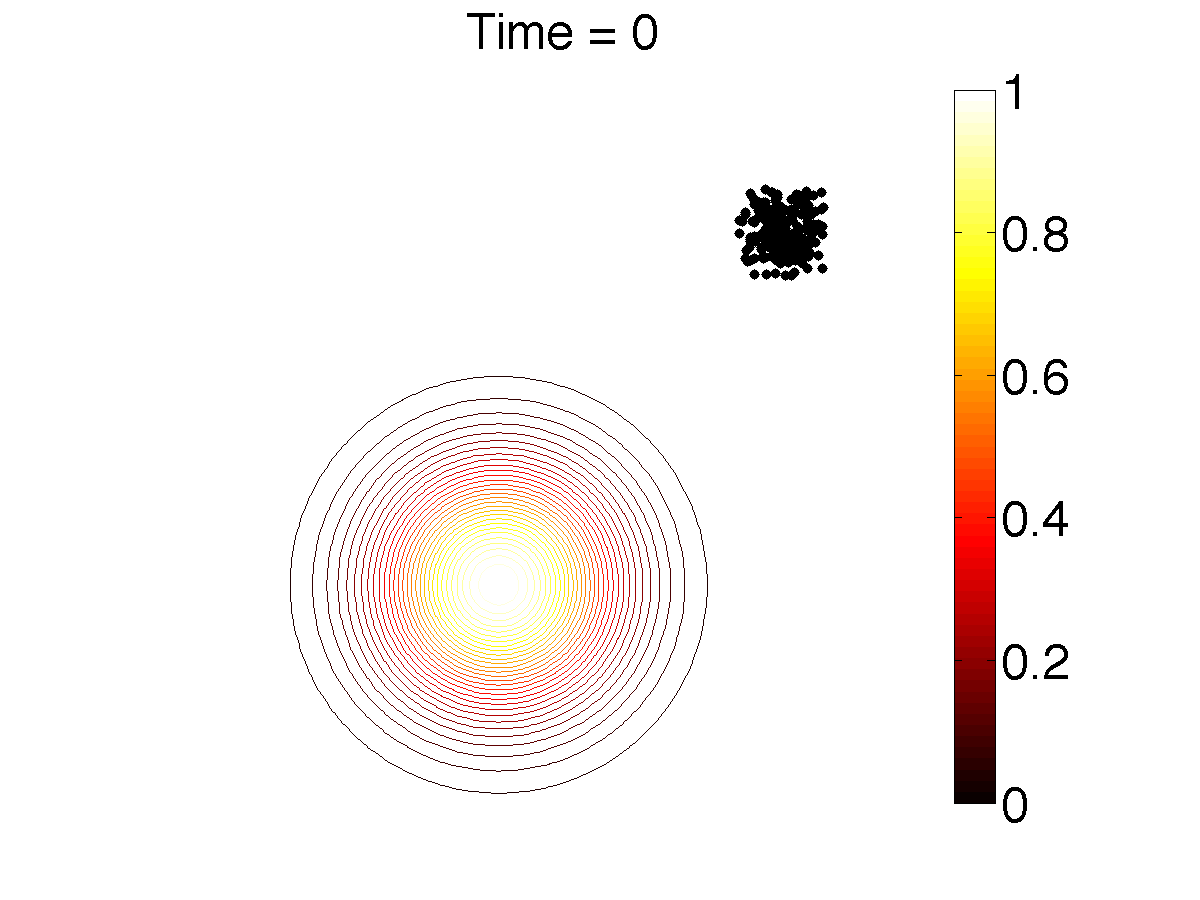
\includegraphics[width=3.25in]{figures/MosqViz_ruleset01_paramset013_run01_001.png} & 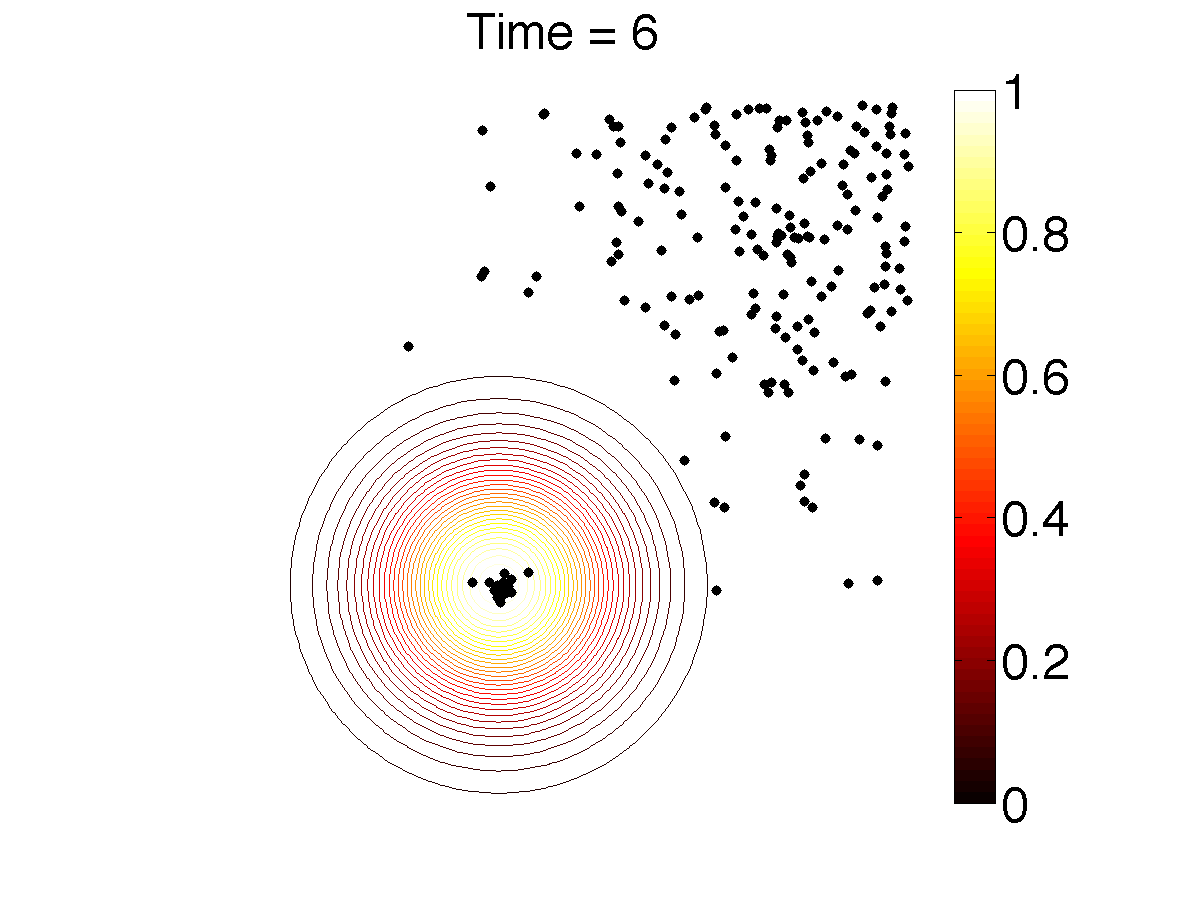
\includegraphics[width=3.25in]{figures/MosqViz_ruleset01_paramset013_run01_025.png}\\
		A & B \\
		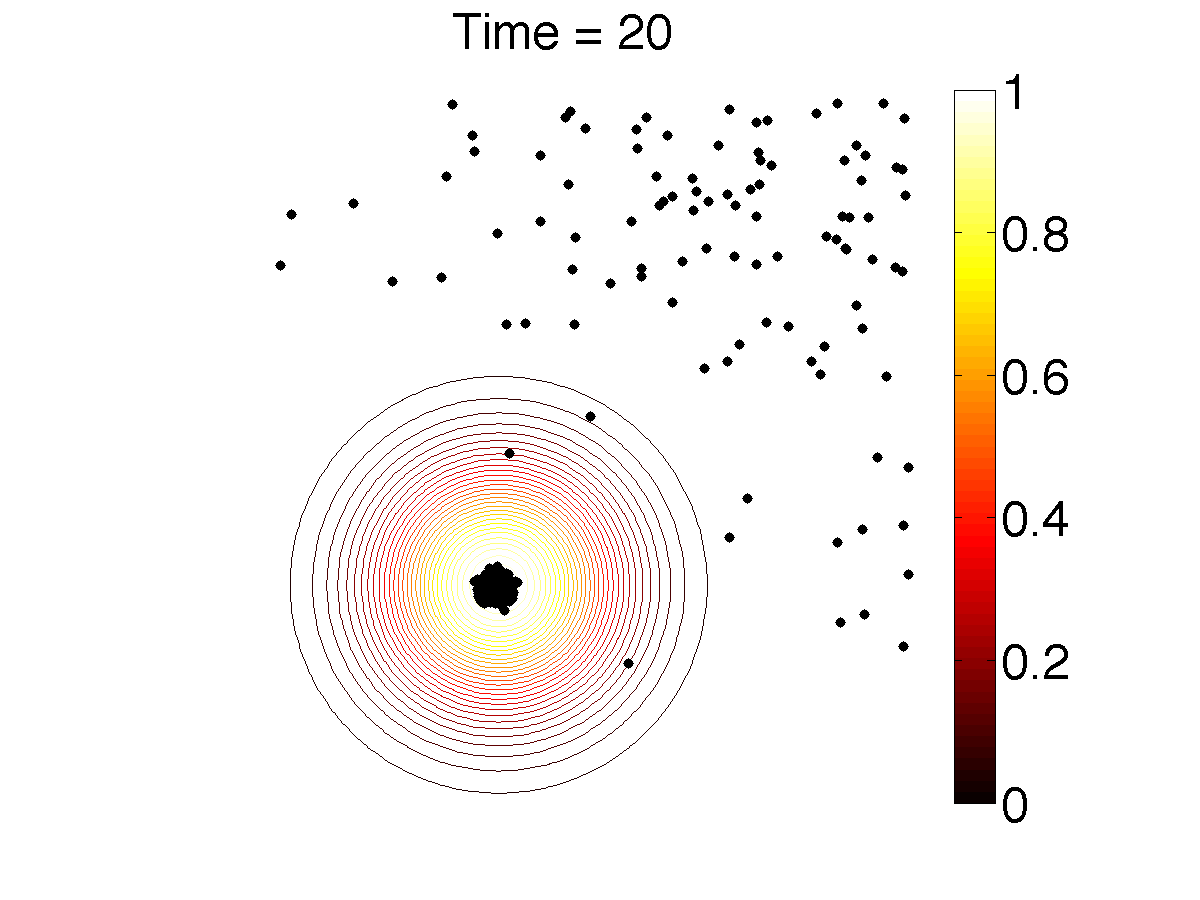
\includegraphics[width=3.25in]{figures/MosqViz_ruleset01_paramset013_run01_061.png} & 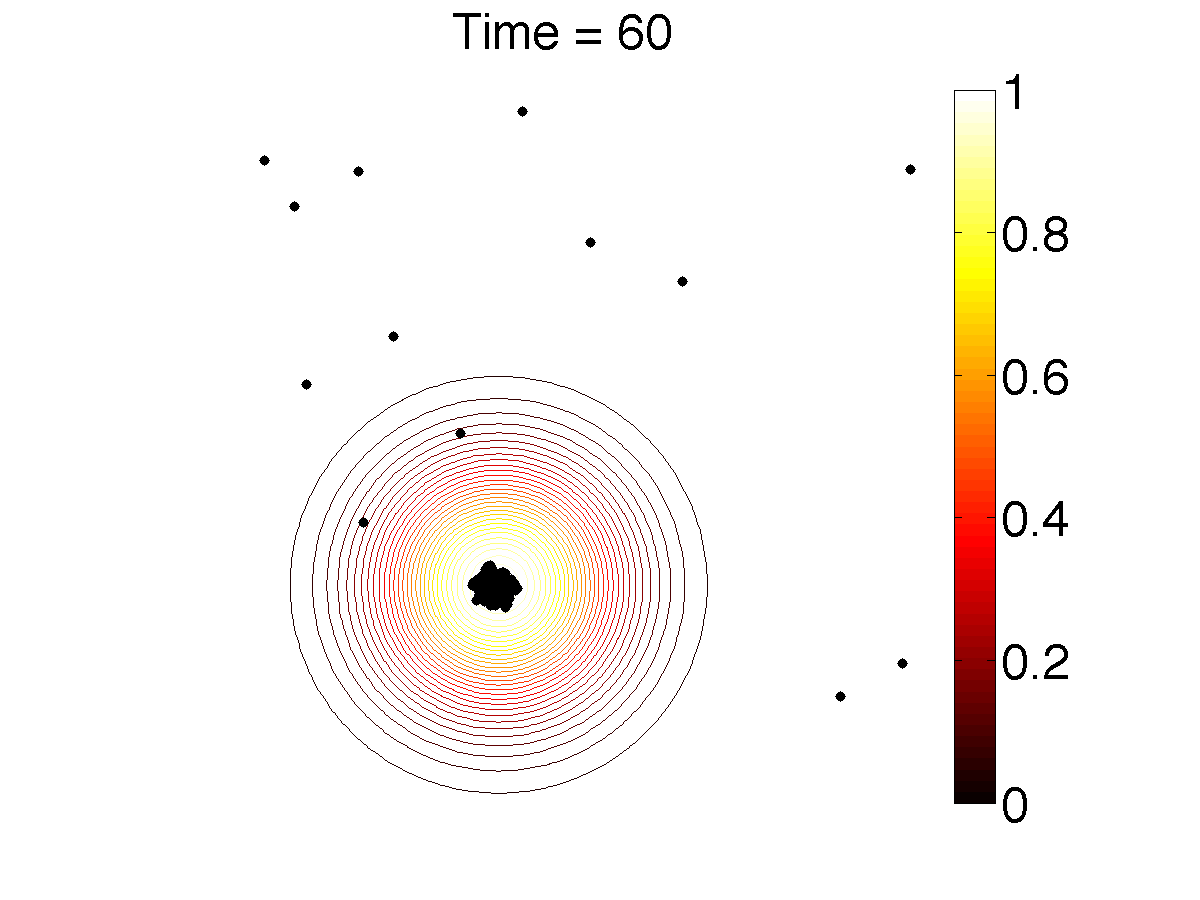
\includegraphics[width=3.25in]{figures/MosqViz_ruleset01_paramset013_run01_111.png}\\
		C & D 
	\end{tabular}
	\caption{Snapshots at various times showing the locations of each of 200 mosquitoes navigating using rule 1 with $\beta_1 = \pi/12$, $S_1 = 0.5$, and $S_2 = 1.25$. The contour plot shows the chemical concentration. Over time, the mosquitoes move from the upper right corner of the domain toward the source center near the lower left, where they maintain irregular flight in the vicinity of the concentration peak. Mosquitoes following different rules may exhibit a larger or smaller group radius around the source. }
	\label{mosqviz}
	\end{figure}

	\textbf{Statistical Comparisons:} We want to know when two rules from Table~\ref{rulesets} result in significantly different behavior. To do this, we use a statistical method described step-by-step below. The heart of our statistical analysis is the two-sided Kolmogorov-Smirnov (KS) test. The KS test is advantageous because it does not require us to know the underlying distribution of mosquitoes, nor it does it require that two different rules have the same type of distribution.
	
	\begin{enumerate}
		\item \textbf{Post-processing:} For ease of analysis, we convert the two dimensional positions of the mosquitoes at each moment in time into distances from the stationary chemical source. This is a reasonable simplification since the concentration is radially symmetric and the mosquito position is only biologically interesting relative to the host. 
		
		We are interested in flight behavior that is mediated by long-range chemical signals and wind. The ``orbiting" behavior about the source visible at later times in Fig.~\ref{mosqviz} is a confounding factor. In the post-processing, we remove mosquitoes from the analysis the first time they appear within a critical radius of the source. We take the critical radius to be $0.012L$, or slightly more than one typical flight length for a mosquito (note that $0.01L = s_0 \Delta t$). Figure~\ref{fig:disthist} shows the distributions of mosquito distances to the source at selected times for two different rules. In the top panel (rule 2), the number of mosquitoes in the domain noticeably decreases with time.
		
		\begin{figure}[htp]
			\begin{center}
				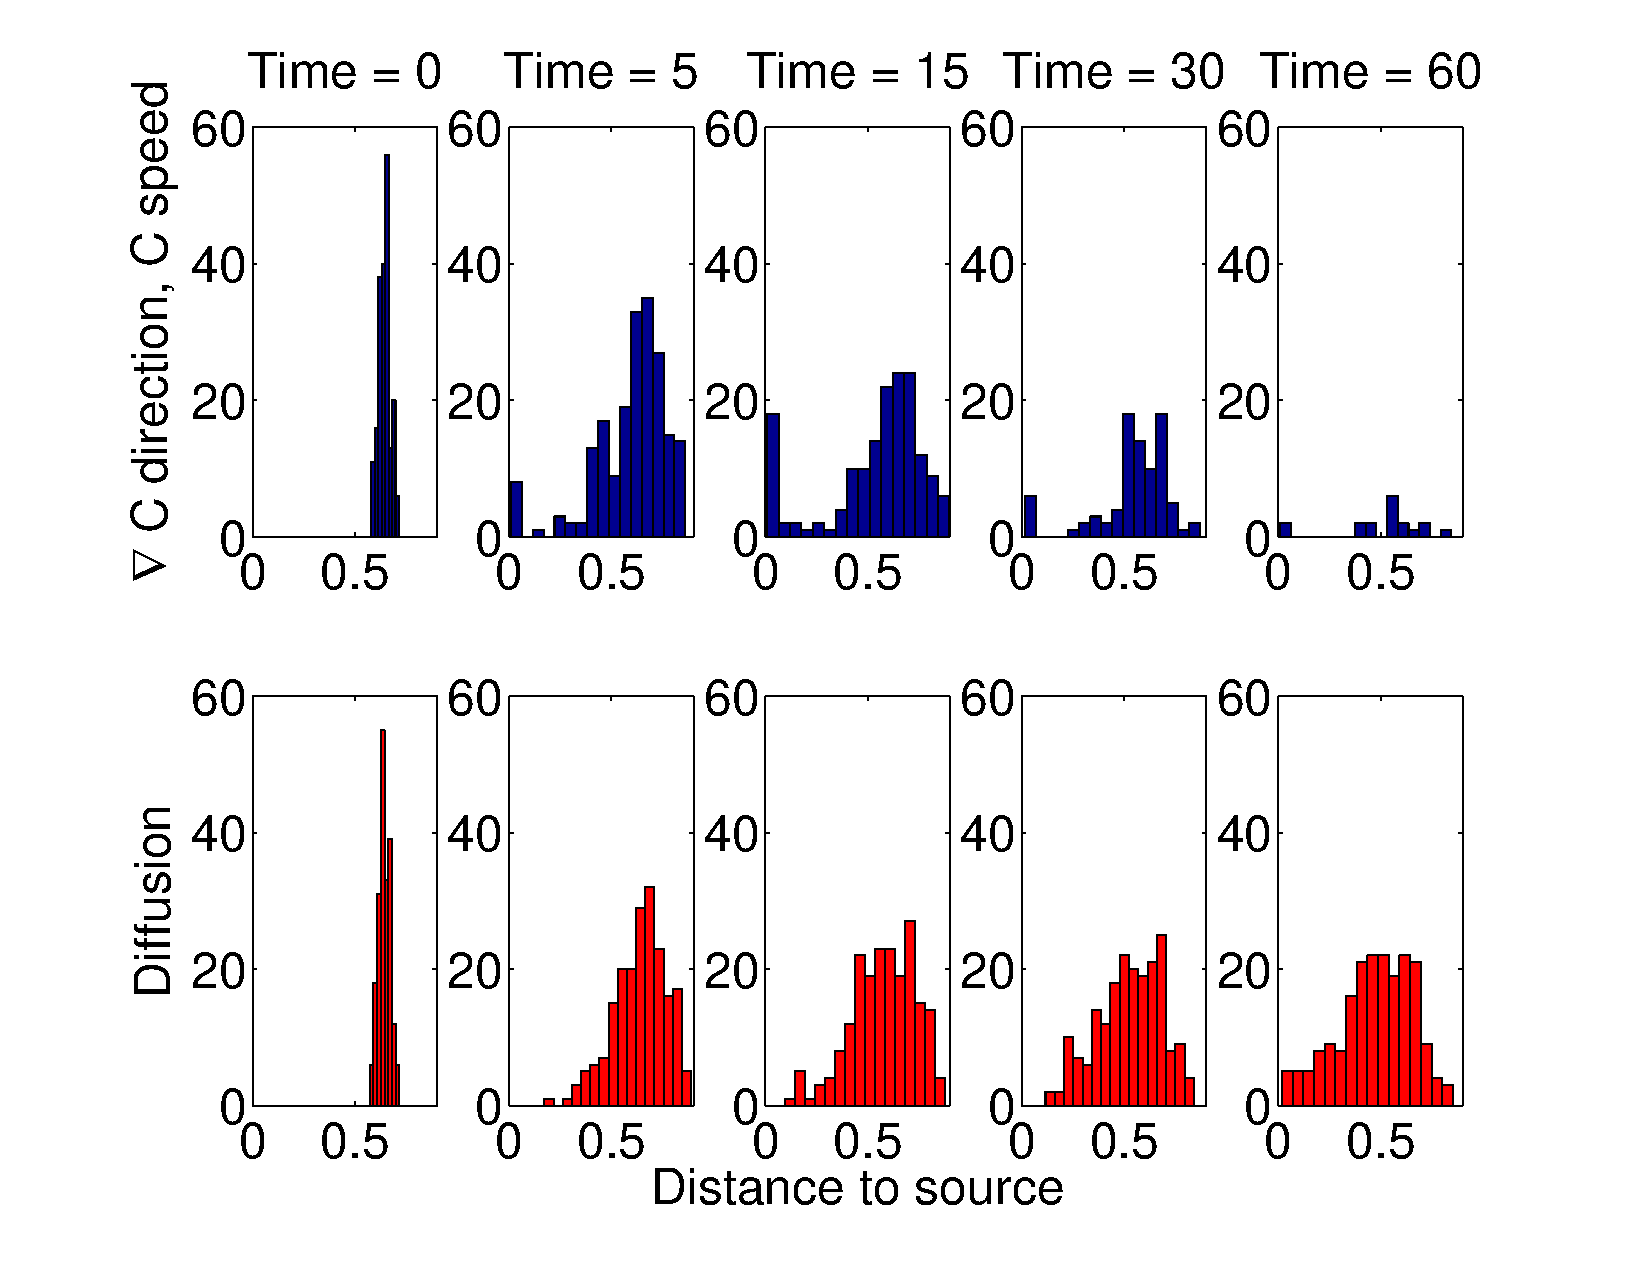
\includegraphics[width=6.5in]{figures/HistogramsRS02PS027Run1_RS10PS001Run1.pdf} 
			\end{center}
			\caption{Histograms of mosquito distances to the chemical source for a rule 2 (chemotaxis; blue) and rule 10 (diffusion; red) at various times from 0 to 60 s. Parameters used for rule 2 are $S_1 =  0.75$ m/s, $ S_2 = 1.25$ m/s, $ \beta_1 = \pi/3,$ and $ \kappa = 0$. The sensory thresholds of CO$_2$ and its gradient are fixed at 0 (i.e., mosquitoes respond to any amount of CO$_2$), and the saturation levels are the maxima over the domain (i.e., mosquito behavior does not exhibit saturation in this test case). The fixed speed for diffusion is 1 m/s. The initial distributions for both rules are similar. There are two major differences between the rules: 1) many mosquitoes have reached the source by time 60 s using rule 2, but few have reached the source under diffusion; and 2) the distribution is bimodal for rule 2 and unimodal (as expected) for diffusion.}
			\label{fig:disthist}
			\end{figure}
					
		\item \textbf{Kolmogorov-Smirnov (KS) statistic:} At each moment in time, we may calculate the KS statistic between distributions of mosquito distances, such as those pictured in Fig.~\ref{fig:disthist}. A schematic describing the calculation of the KS statistic is shown in Fig.~\ref{fig:kstut}, using $t = 30$ from the panels in Fig.~\ref{fig:disthist}. There are three steps: first, build cumulative distribution functions (CDFs) for each rule; second, normalize them by the number of remaining mosquitoes; and third, find the maximum difference between the two normalized CDFs. The maximum difference is the KS statistic, which is bounded between 0 and 1. 
		
		\begin{figure}[htp]
			\begin{center}
				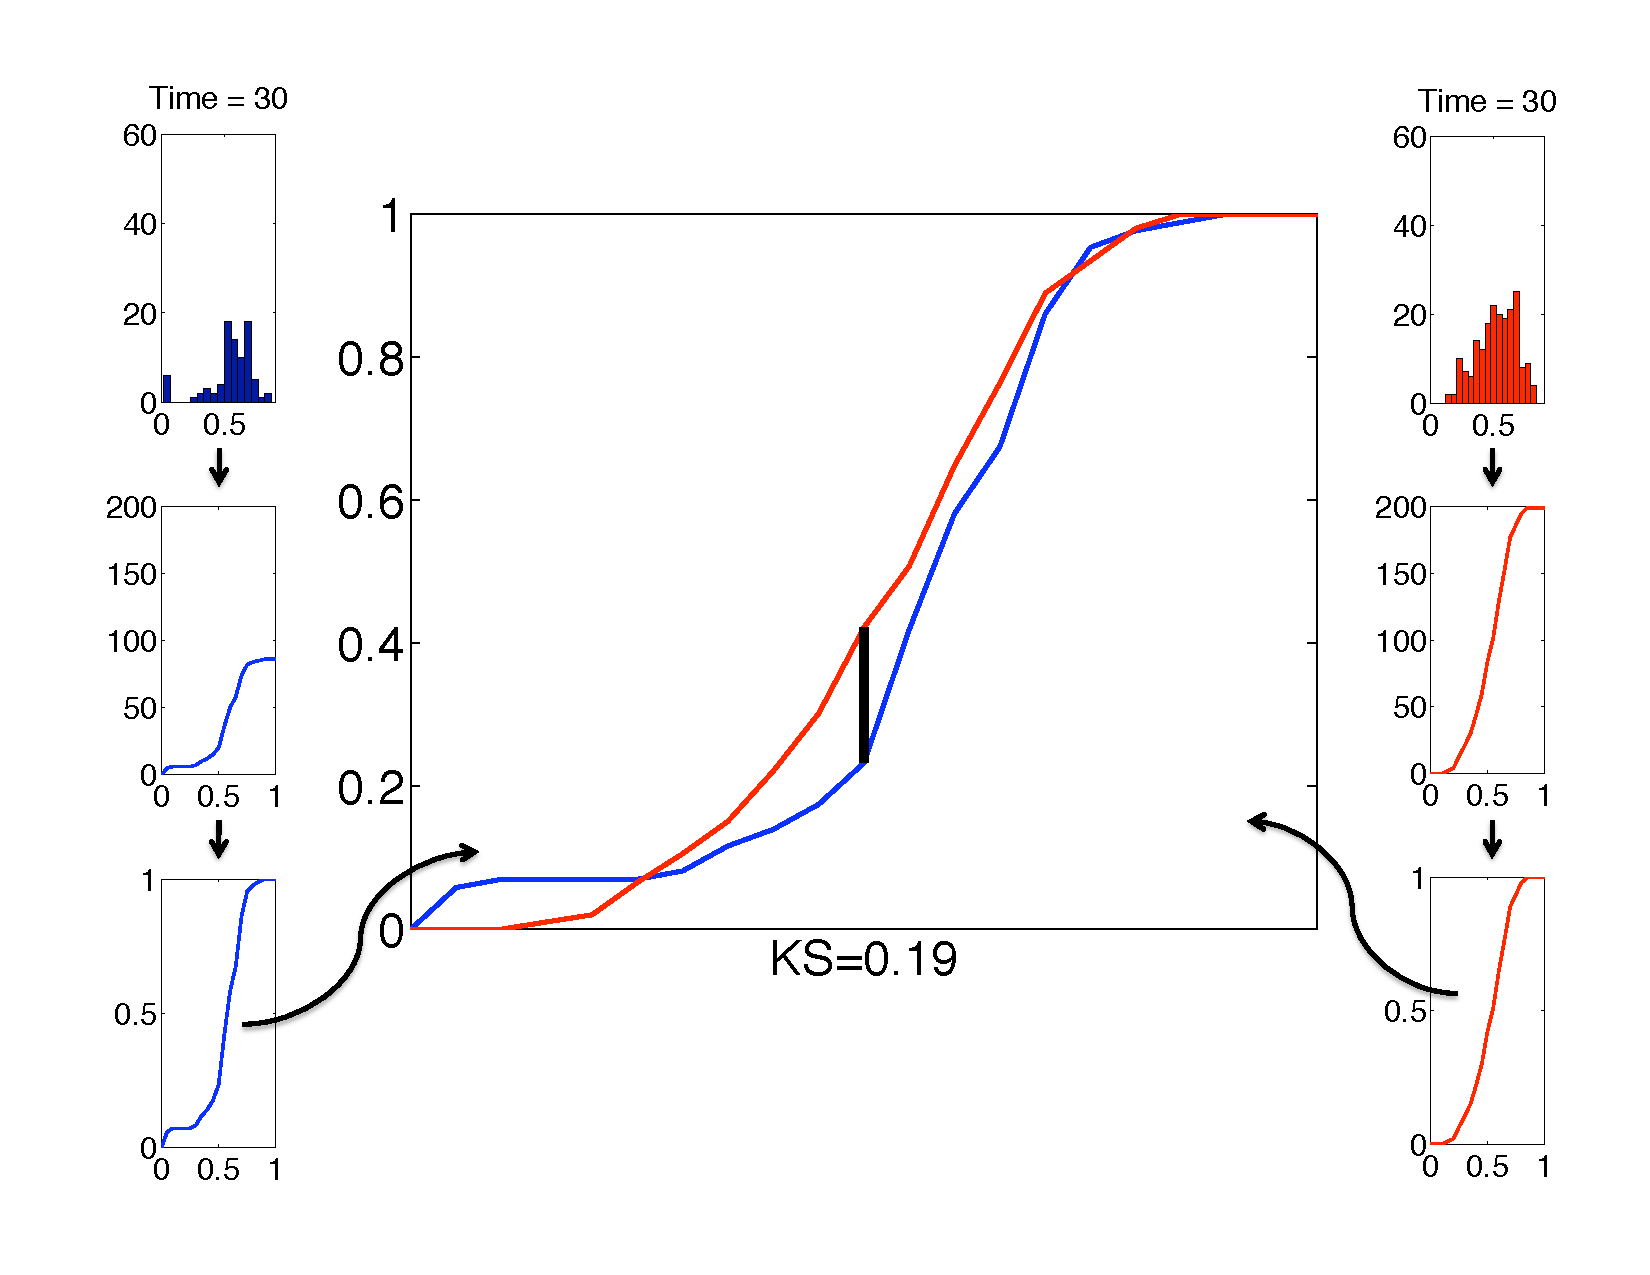
\includegraphics[width=6.5in]{figures/KStutorial.pdf} 
			\end{center}
			\caption{Schematic of the KS statistic calculation. First, a CDF is constructed from the mosquito distances to the source. Then the CDF is normalized. CDFs from two different rules at the same time are compared, and the largest difference between them is the KS statistic.}
			\label{fig:kstut}
			\end{figure}
		
			\item \textbf{Empirical distributions from repeated simulations:} We must develop an expectation for the behavior of the KS statistic \emph{within} a rule in order to compare \emph{between} rules. To do this, we calculate all the independent pairwise KS statistics between the 25 simulations that we ran for each rule and parameter set (a total of 25(25-1)/2 = 300 KS statistics). We take the mean of this collection at each moment in time, and estimate the 95\% confidence interval using the 7th and 293rd largest values. The empirical distribution of KS statistics for diffusion is in Fig.~\ref{fig:diffempdist} (red lines). Notice that the mean and confidence interval are quite stationary. 
			
			\begin{figure}[htp]
				\begin{center}
					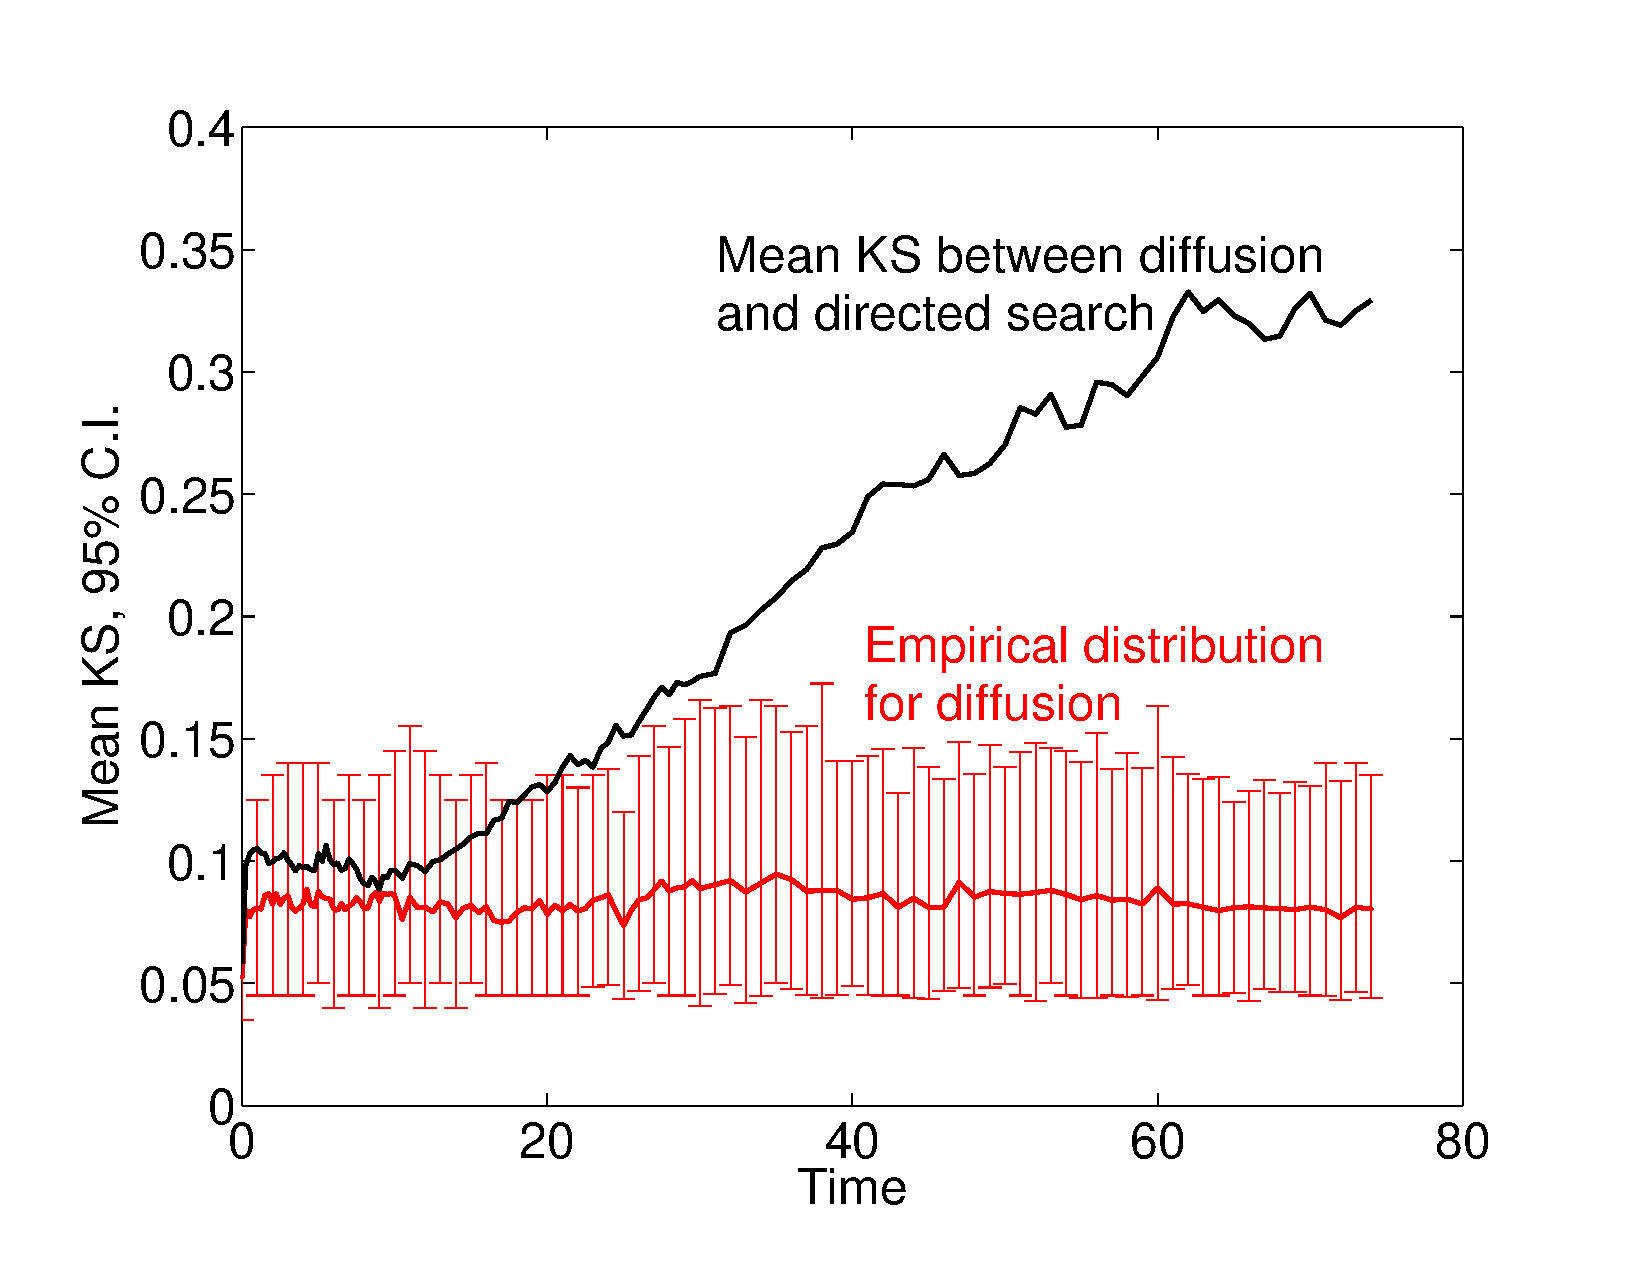
\includegraphics[width=3.5in]{figures/DiffusionDirectedSearchComp.pdf}
				\end{center}
				\caption{Mean KS statistics between rule 2 and diffusion (black line) compared to the empirical distribution of KS statistics from diffusion (red lines); mean and 95\% confidence interval. The two rules clearly result in significantly different behaviors at late times.}
				\label{fig:diffempdist}
				\end{figure}
			
			
			\item \textbf{Comparing mean KS statistics:} We are now prepared to assess the difference between two rule sets. Each has 25 simulations, so we calculate all pairwise KS statistics between them (625 KS statistics). We only do the calculations as long as both rule sets have at least 10 mosquitoes in \emph{every} simulation. We take the mean of this collection at each moment in time and compare it to the empirical distribution with the tighter confidence interval. The example comparison that we have been tracking, rule 2 vs diffusion, is shown in Fig.~\ref{fig:diffempdist}.B. Happily, there is a significant difference between diffusion and rule 2. Shortly after time 75, one of the simulations drops below the required 10 mosquitoes and the comparison ends. 
			
	\end{enumerate}
	
	Using this methodology, we have discovered that the choice of sensory modality underlying the agents' heuristic is not critical to the modeling process. By choosing parameters appropriately, we are able to produce mosquito behavior (in aggregate) that is indistinguishable between rule sets. Figure~\ref{fig:goodmatches} shows our two best matches to rule 2 -- rules 1 and 6. The similarity between these heuristics appears to be robust to minor perturbations (see Appendix~\ref{app:perturb}). The other rule sets exhibit acceptable to poor matches to rule 2, despite our attempts to optimize parameters. See Appendix~\ref{app:rule2matches} for these other comparisons. Lastly, we also tested to see if changing the concavity of the response function Eq.~\eqref{eqn:functional} or the saturation level of the agent senses changed the agent behavior, and found no significant differences (Appendix~\ref{app:kappa}).
	
	\begin{figure}[hbp]
		\begin{center}
			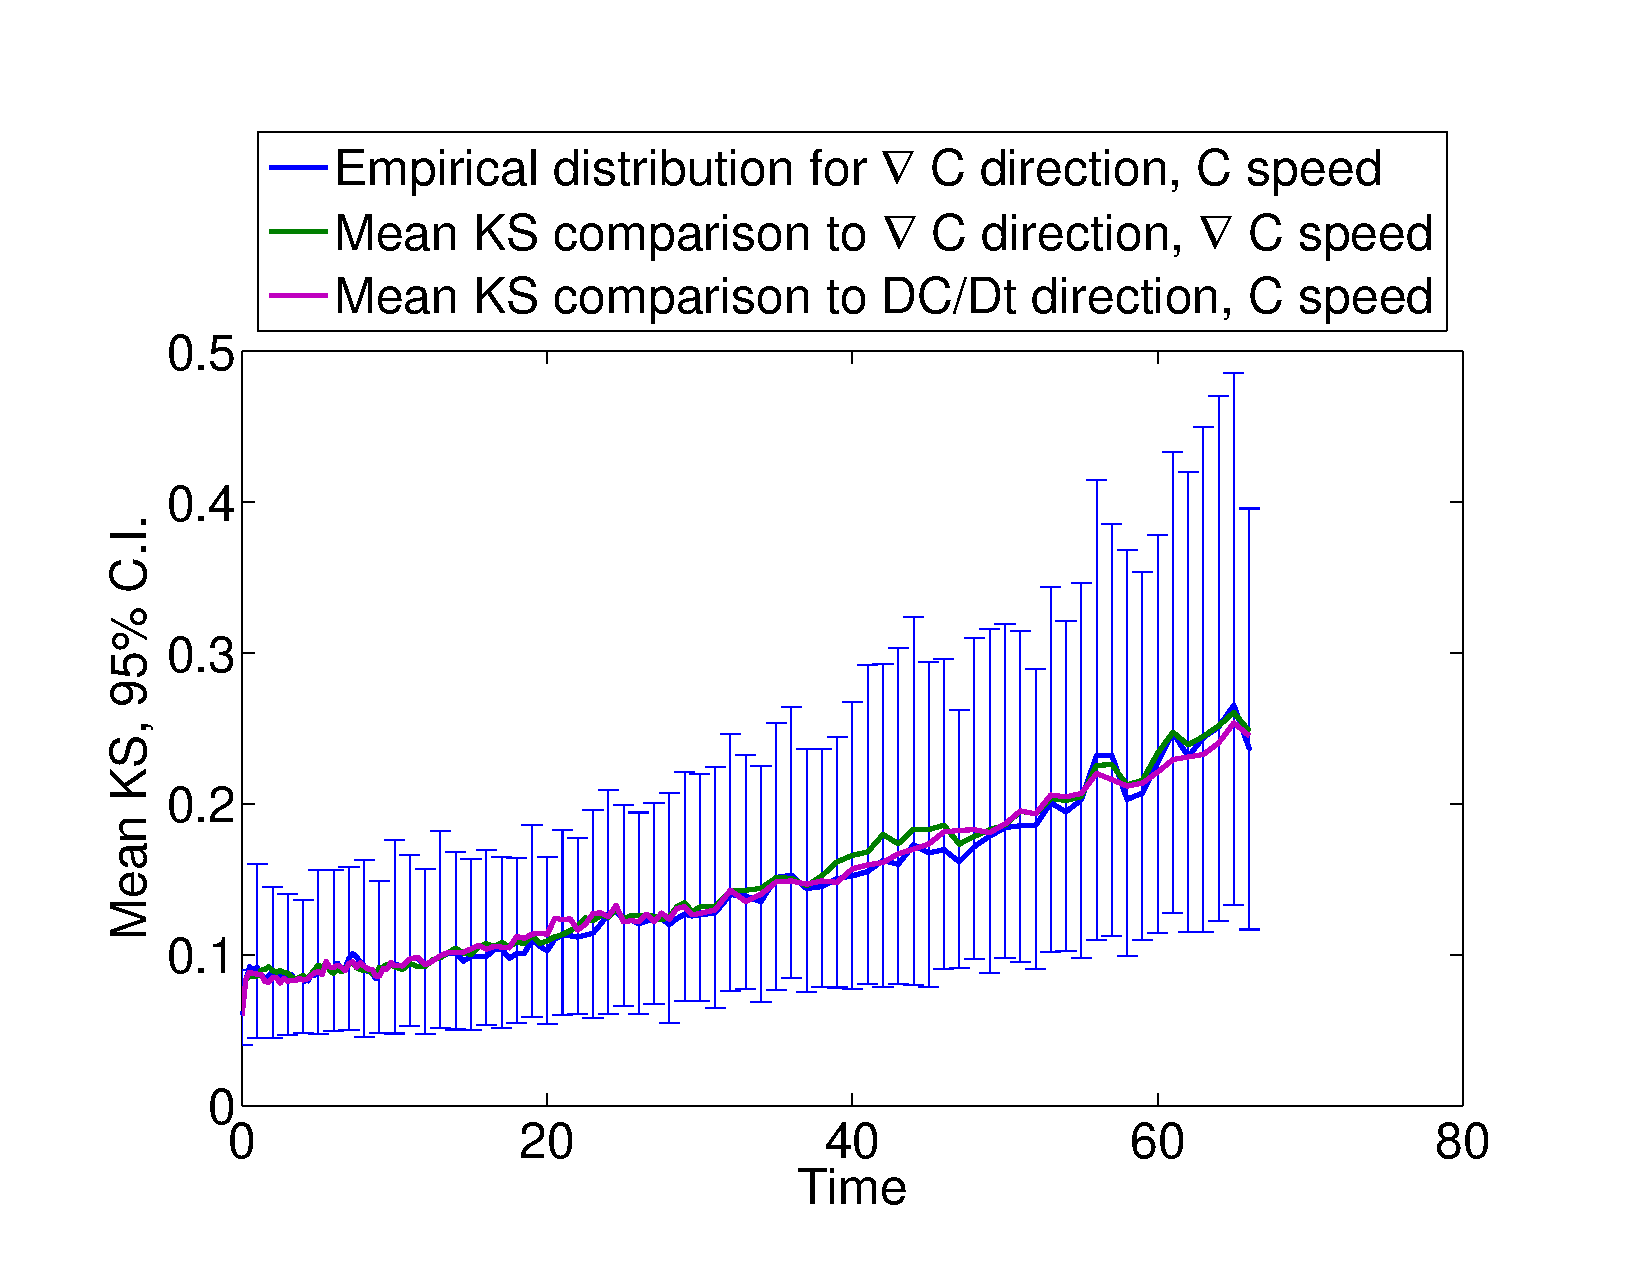
\includegraphics[width=4.0in]{figures/GoodComparisonsRS02PS027_RS01PS13_RS06PS12.pdf} 
		\end{center}
		\caption{Mean KS statistics for rule 2 vs rule 1 (green line) and rule 2 vs rule 6 (magenta line). The empirical distribution used for the comparison is for rule 2 (blue lines). Parameters used for rule 2 are $S_1 =  0.75$ m/s, $ S_2 = 1.25$ m/s, and $ \beta_1 = \pi/3$; for rule 1 are $S_1 =  0.5$ m/s, $ S_2 = 1.25$ m/s, $ \beta_1 = \pi/12$; and for rule 6 are $S_1 =  0.5$ m/s, $ S_2 = 1.25$ m/s, $ \beta_1 = 0$.}
		\label{fig:goodmatches}
		\end{figure}
	
	
	
		
	\subsubsection{Response to CO$_2$: Final choice of heuristics}
	
	Given that the underlying sensory modality of the heuristic is not critical, we choose to implement rule 2 for its convenience. Each mosquito is given an entry location and time into the simulated domain and afterwards controls its direction and speed at every nondimensional time step $\Delta t = 0.01$. 
	The speed of a mosquito is constant during ranging flight and determined by absolute CO$_2$ concentration during homing flight:
	\[
	s(x,y,t) =   \left\{\begin{matrix} s_0, & C < C_0 \\ F(\,C(x,y,t);S_1,S_2\,), & C \geq C_0 . \end{matrix} \right.
	\hskip20pt
	\]
	This formulation limits an agent's speed to the interval $[S_1,S_2]$, with $s$ decreasing as $C$ increases. 
	
	
	When $C \geq C_0$ and $\theta_c$ denotes the direction of $\nabla C$ at $(x,y)$ and time $t$, a new chemotactic direction of motion is calculated according to
	\begin{eqnarray*}
	\beta &=& F(\, \nabla C(x,y,t);\beta_1,\beta_2\,) \\
	\Theta_c &=&  \theta_c + \eta\beta.
	\end{eqnarray*}	
	In total, the new agent position is 
	\begin{equation*}
	\left.\begin{pmatrix} x \\ y \end{pmatrix}\right\vert_{t+\Delta t} = \left.\begin{pmatrix} x \\ y \end{pmatrix}\right\vert_{t} + s(x,y,t) \Delta t \begin{pmatrix} \gamma\cos\Theta_v + (1-\gamma)\cos\Theta_c \\ \gamma\sin\Theta_v + (1-\gamma)\sin\Theta_c \end{pmatrix} + \vec V \Delta t
	\end{equation*}
	where the last term is passive advection and $\gamma$ is a free parameter denoting the relative weight of wind vs CO$_2$ importance during the mosquito host-seeking stage:
	\[
	\gamma =  \left\{\begin{matrix} 1, & C < C_0 \\ \gamma_0 \in [0,1], & C \geq C_0 .\end{matrix} \right. 
	\hskip20pt
	\]
	 
	\subsection{Full system of equations}
		
		\begin{eqnarray*}
			\frac{\partial C}{\partial t} + {\vec V}\cdot\nabla C &=& D\nabla^2 C + S(x,y) \\
			\alpha &=& F(\,\vec V(x,y,t);\alpha_1,\alpha_2\,) \\
			\Theta_v &=&  \left\{\begin{matrix}\theta_v + \psi + \eta\alpha, & C < C_0, & \text{$\psi$ varies with wind strategy} \\  \theta_v + \pi + \eta\alpha, & C \geq C_0, & \text{upwind strategy} \qquad \end{matrix}\right. \\ 
			\beta &=& F(\, \nabla C(x,y,t);\beta_1,\beta_2\,) \\
			\Theta_c &=&  \theta_c + \eta\beta \\
			s(x,y,t) &=&   \left\{\begin{matrix} s_0, & C < C_0 \\ F(\,C(x,y,t);S_1,S_2\,), & C \geq C_0 \end{matrix} \right.\\
			\gamma &=&  \left\{\begin{matrix} 1, & C < C_0 \\ \gamma_0 \in [0,1], & C \geq C_0 .\end{matrix} \right. \\
			\left.\begin{pmatrix} x \\ y \end{pmatrix}\right\vert_{t+\Delta t} &=& \left.\begin{pmatrix} x \\ y \end{pmatrix}\right\vert_{t} + s(x,y,t) \Delta t \begin{pmatrix} \gamma\cos\Theta_v + (1-\gamma)\cos\Theta_c \\ \gamma\sin\Theta_v + (1-\gamma)\sin\Theta_c \end{pmatrix} + \vec V \Delta t
		\end{eqnarray*}
			
	


	\section{Results}
	\begin{itemize}
		\item Simulations varying mosquito ranging flight behavior (crosswind, downwind, upwind).
		\item Simulations varying the number of hosts in each group or the volume in which there are a fixed number of hosts (can do this with one and two groups).
		\item Plots of resultant per capita biting rate with respect to ranging flight behavior and host density (and host location within a group?).
		\item Other measures of heterogeneity -- Ivo?
	\end{itemize}

	\section{Discussion/Conclusions}
	\begin{itemize}
		\item Discuss applicability of results to parameter choice in current models of vector-borne diseases.
		\item Future directions, two possibilities:
		\begin{itemize}
			\item Couple to a longer time scale model that incorporates transmission, host movement, infection, and death for explicit small scale modeling of disease spread.
			\item Model more complex scenarios (gusting wind, moving hosts, breathing rate) in order to further enhance parameter choice for broader scale SIR models.
		\end{itemize}
	\end{itemize}


\appendix 

\section{Robustness to perturbations}\label{app:perturb}

Here we perform a minor perturbation to the chemical gradient to see how robust our matches from Fig.~\ref{fig:goodmatches} are. We add a small bump to the concentration gradient centered at (0.3, 0.75) that is one-tenth the height of the original, which is still located at (0.4, 0.3). The new chemical concentration is pictured in Fig.~\ref{mosqvizperturb} along with the positions of 200 mosquitoes at various times. Agent paths to the source are shifted toward the perturbation as opposed to the unperturbed case in Fig.~\ref{mosqviz}.

\begin{figure}[htp]
\begin{tabular}{cc}
	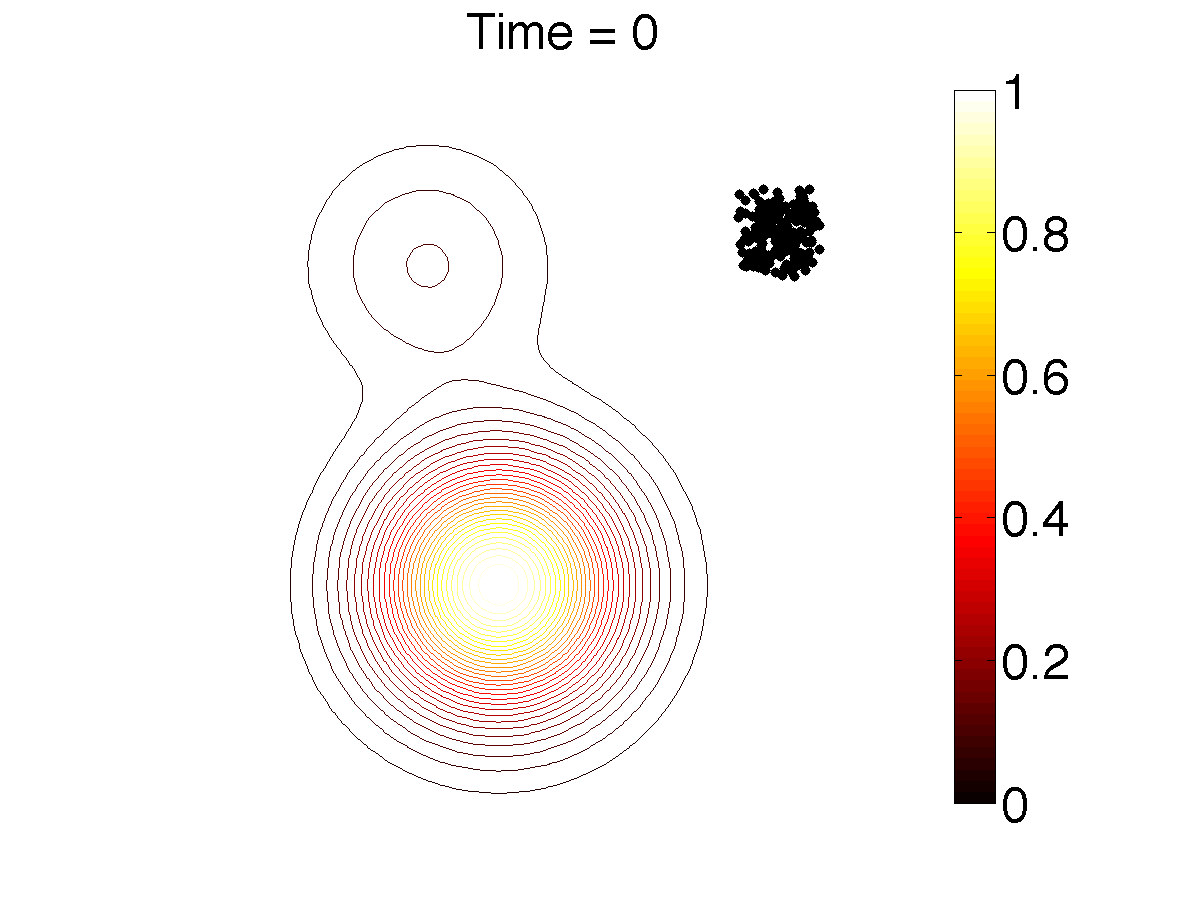
\includegraphics[width=3.25in]{figures/MosqVizPerturb_ruleset01_paramset013_run01_001.png} & 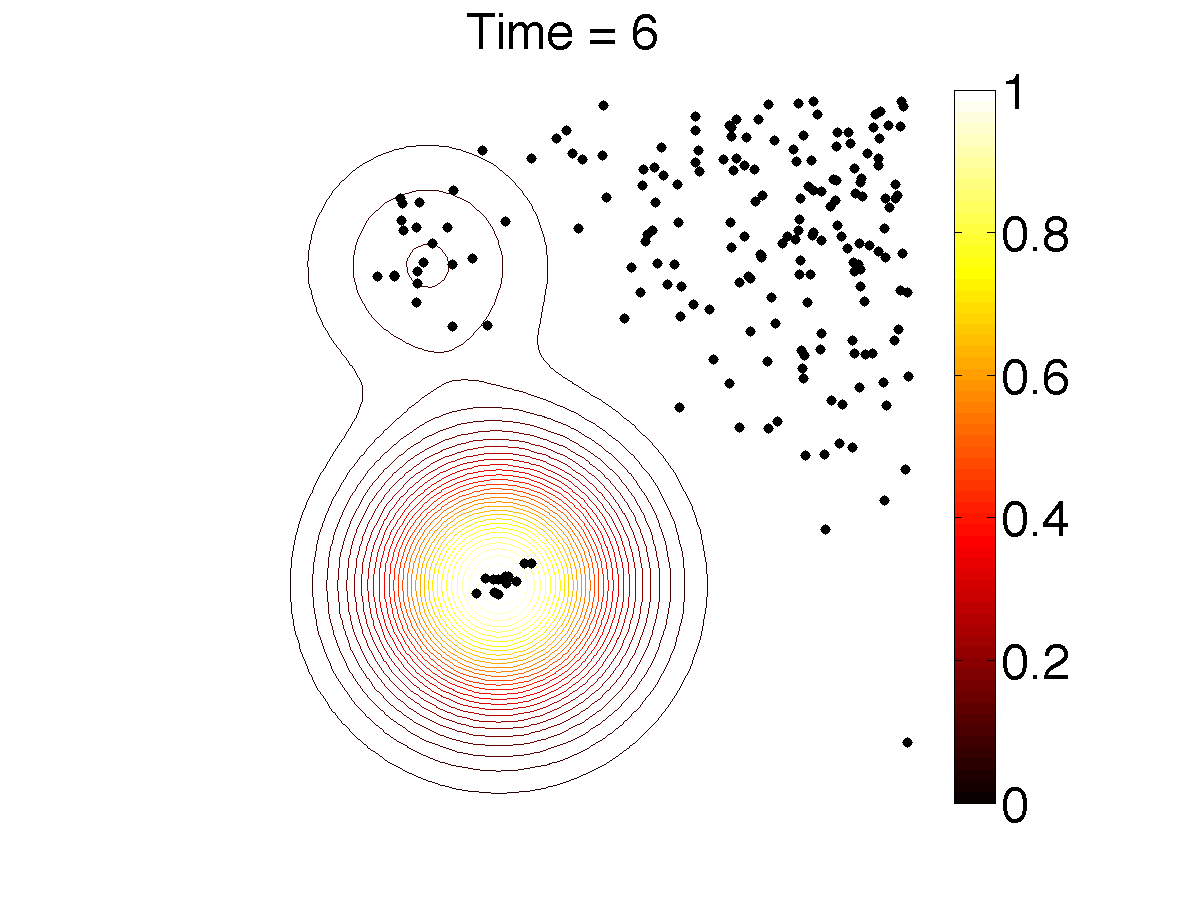
\includegraphics[width=3.25in]{figures/MosqVizPerturb_ruleset01_paramset013_run01_025.png}\\
	A & B \\
	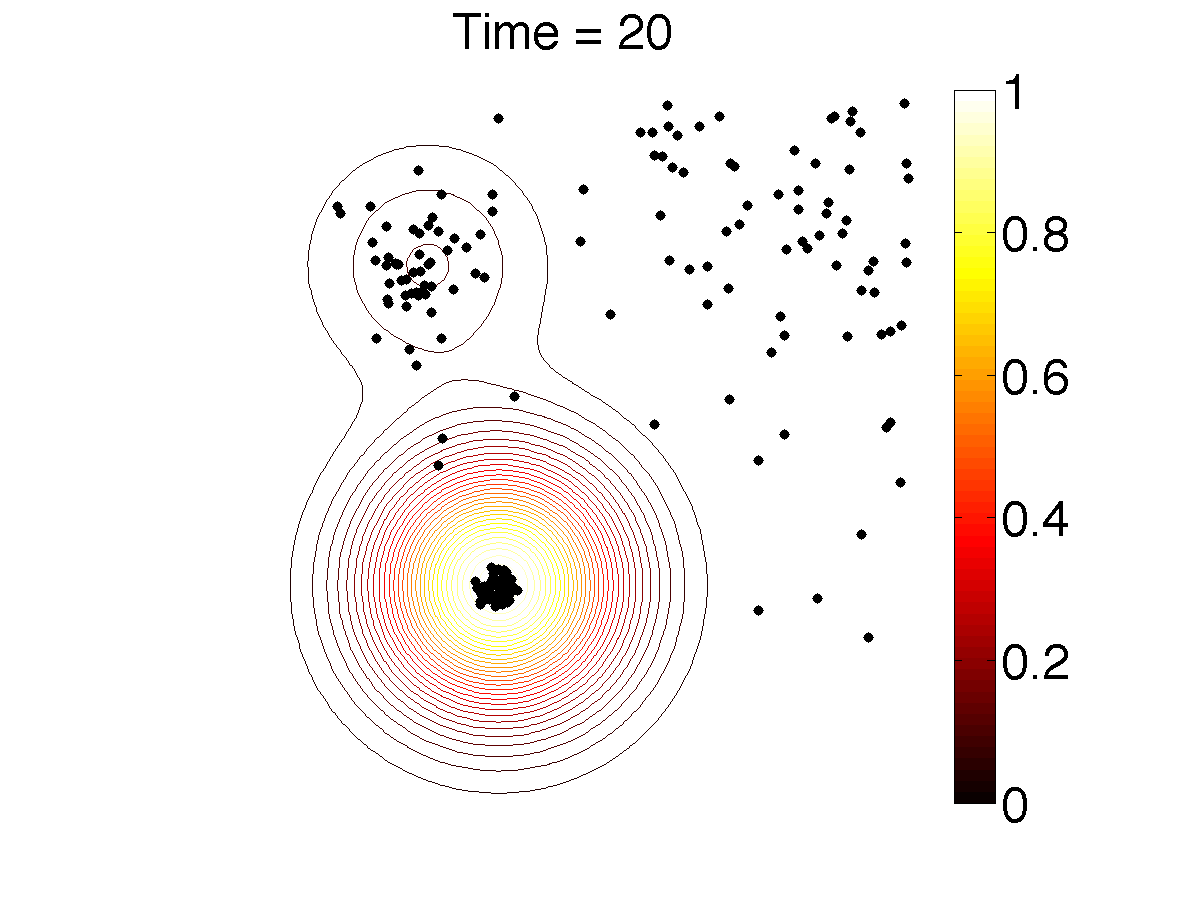
\includegraphics[width=3.25in]{figures/MosqVizPerturb_ruleset01_paramset013_run01_061.png} & 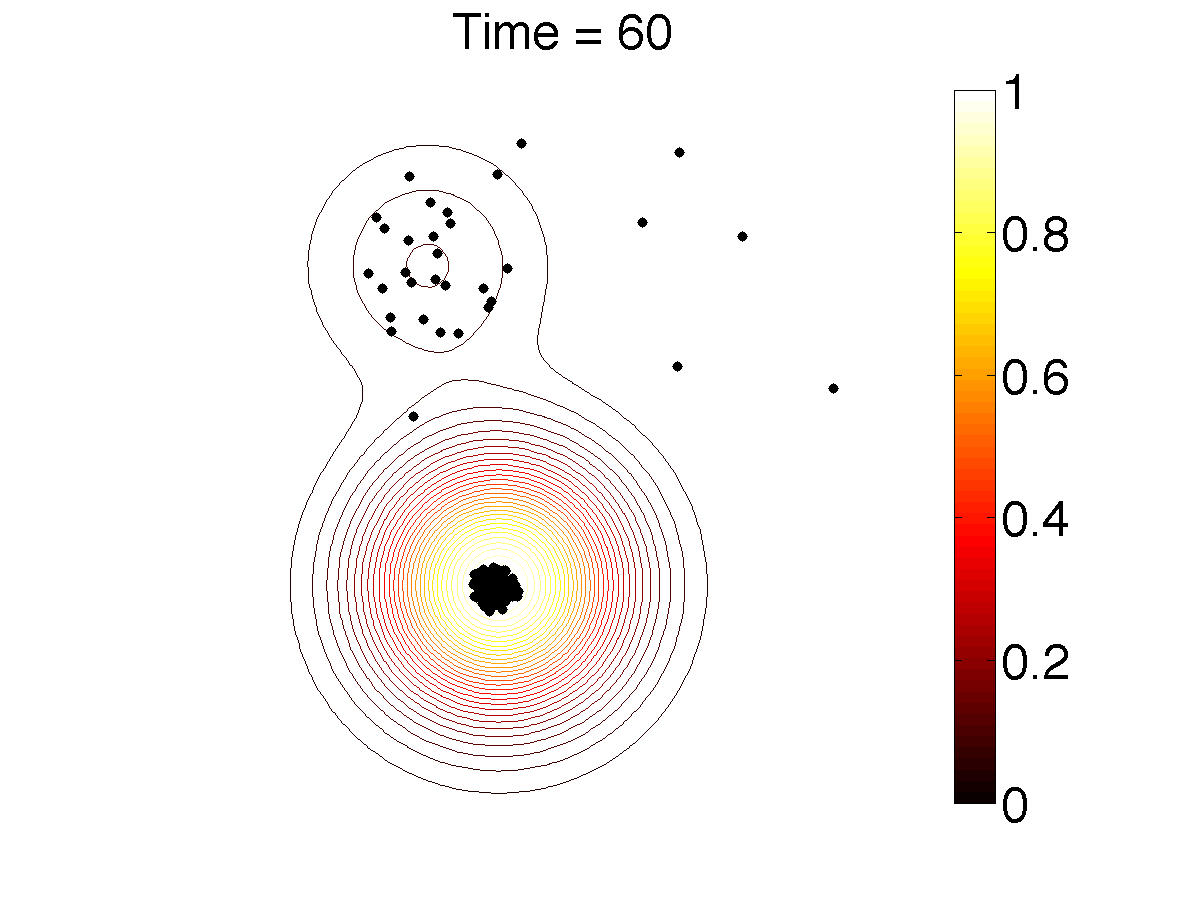
\includegraphics[width=3.25in]{figures/MosqVizPerturb_ruleset01_paramset013_run01_111.png}\\
	C & D 
\end{tabular}
\caption{Snapshots at various times showing the locations of each of 200 mosquitoes navigating using rule 1 with $\beta_1 = \pi/12$, $S_1 = 0.5$, and $S_2 = 1.25$. The contour plot shows the double-bump chemical concentration. The mosquito agents are clearly influenced by the presence of the second concentration bump.}
\label{mosqvizperturb}
\end{figure}


The best matches to rule 2 were rules 1 and 6 with the parameter sets indicated in the caption in Fig.~\ref{fig:goodmatches}. We re-examine these matches under the perturbed chemical concentration in Fig.~\ref{mosqvizperturb}. The mean KS statistics are shown in Fig.~\ref{ksperturb}, and it can be seen the match with rule 6 is still very good, and the match with rule 1 is still reasonable, although poorer. We conclude that matching rules are reasonably robust to small perturbations.

\begin{figure}[htp]
\begin{tabular}{cc}
	\multicolumn{2}{c}{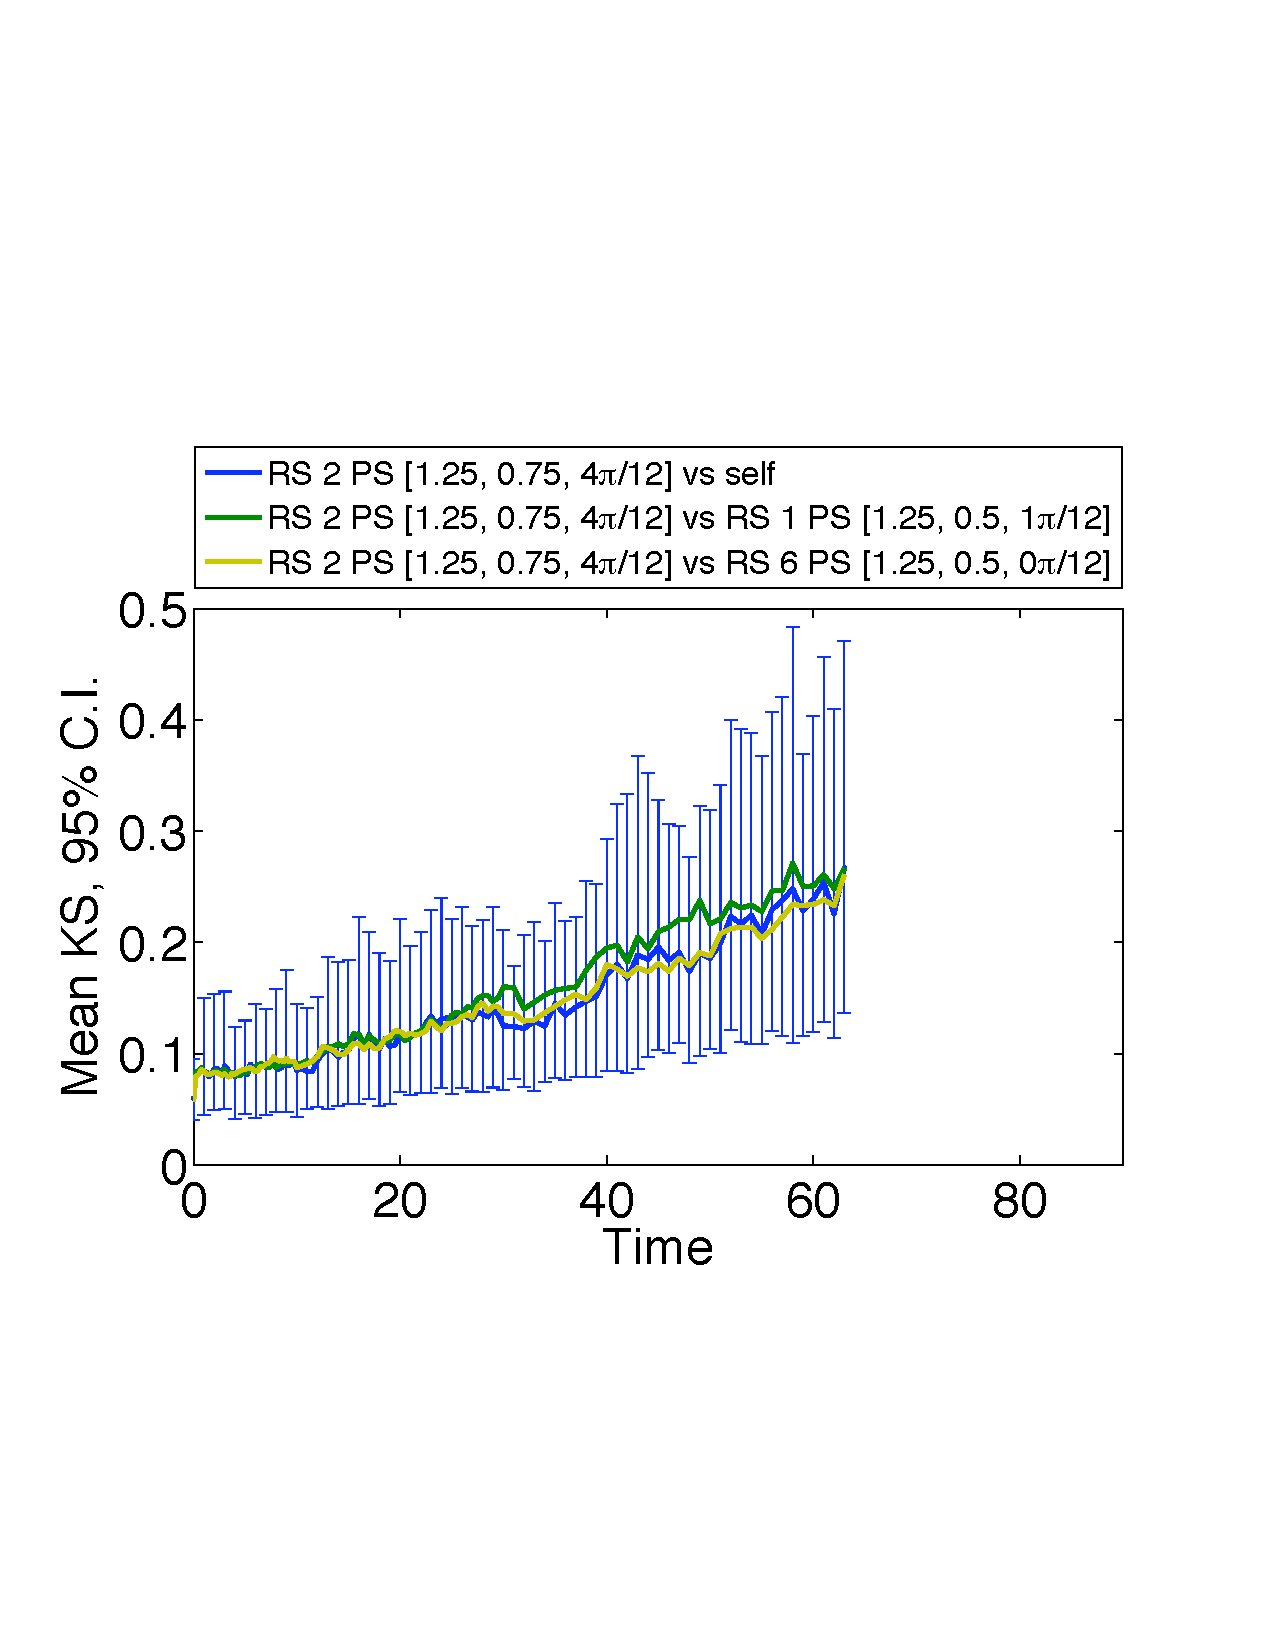
\includegraphics[width=3.25in]{figures/KSstatPerturb_RS02PS027_vs_RS01PS013_RS06PS012.pdf}} \\
	\multicolumn{2}{c}{A} \\
	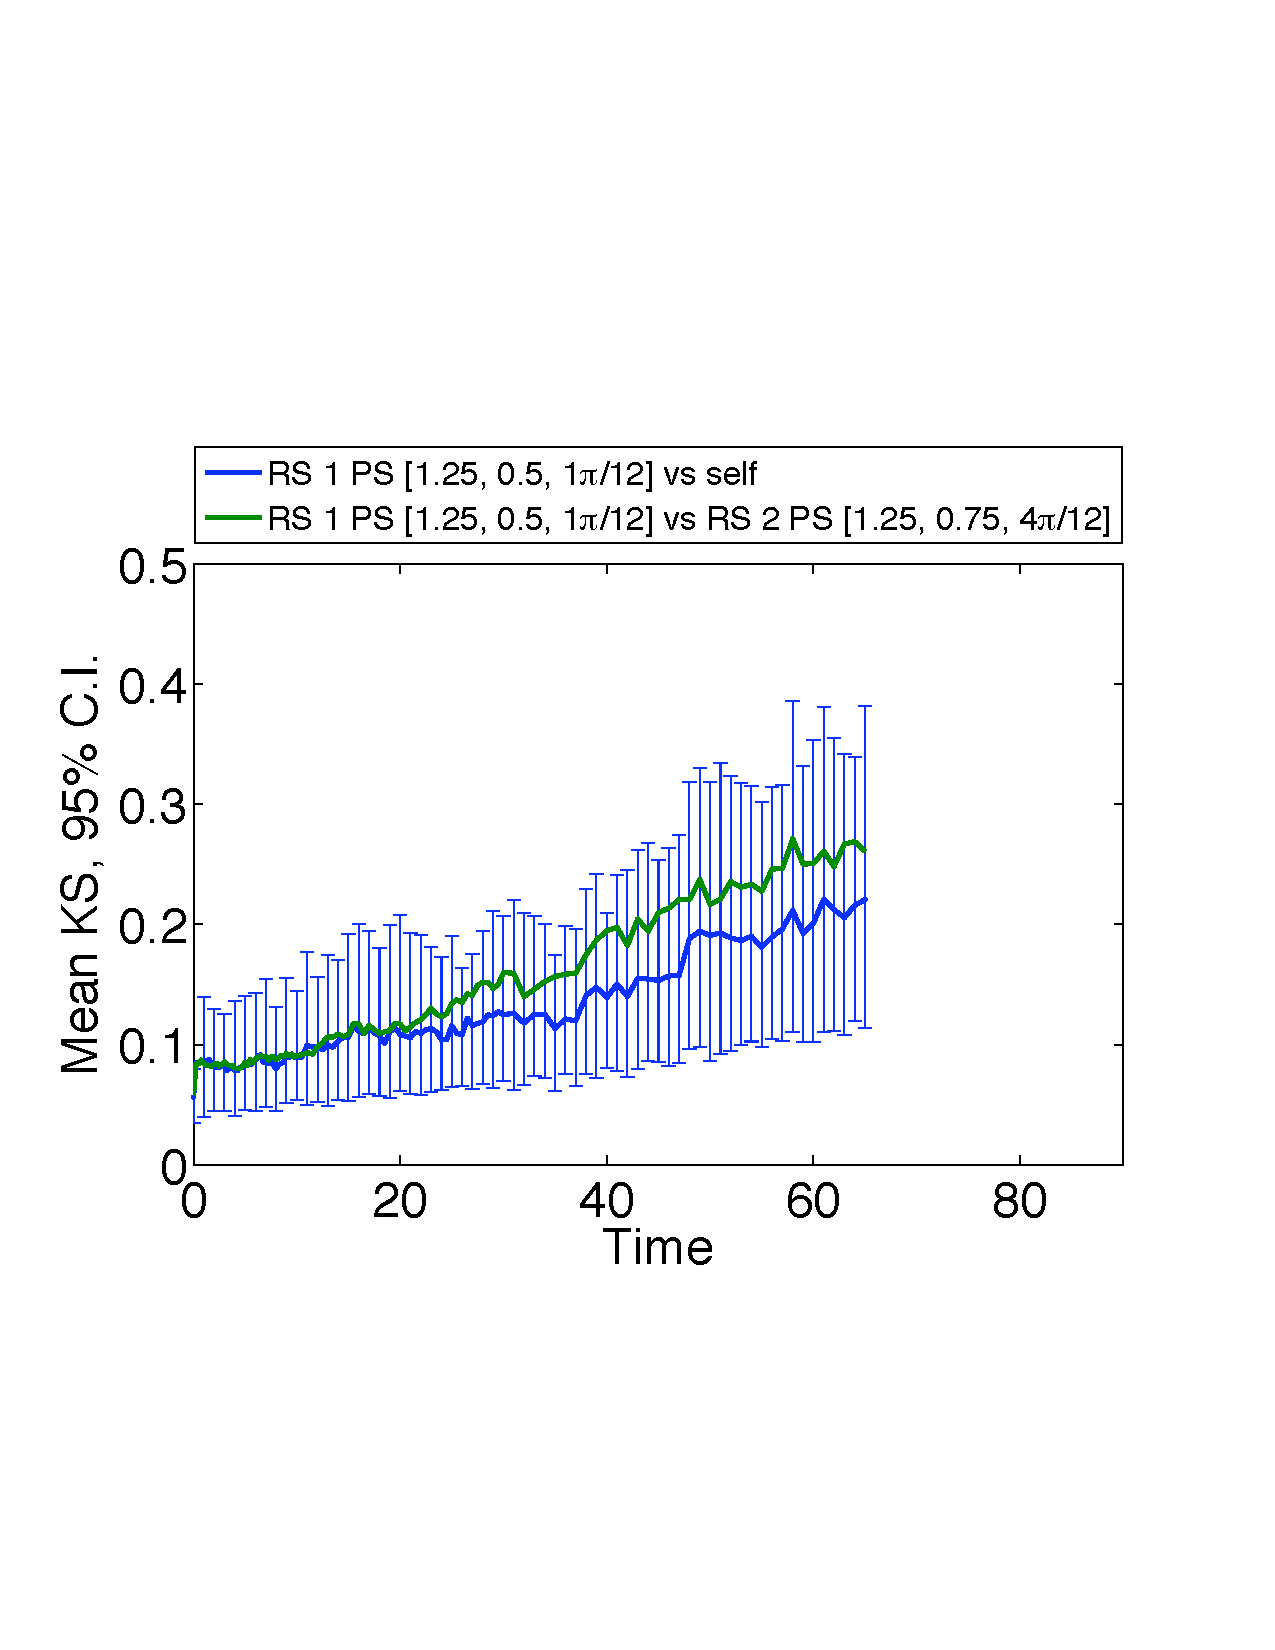
\includegraphics[width=3.25in]{figures/KSstatPerturb_RS01PS013_vs_RS02PS027.pdf} & 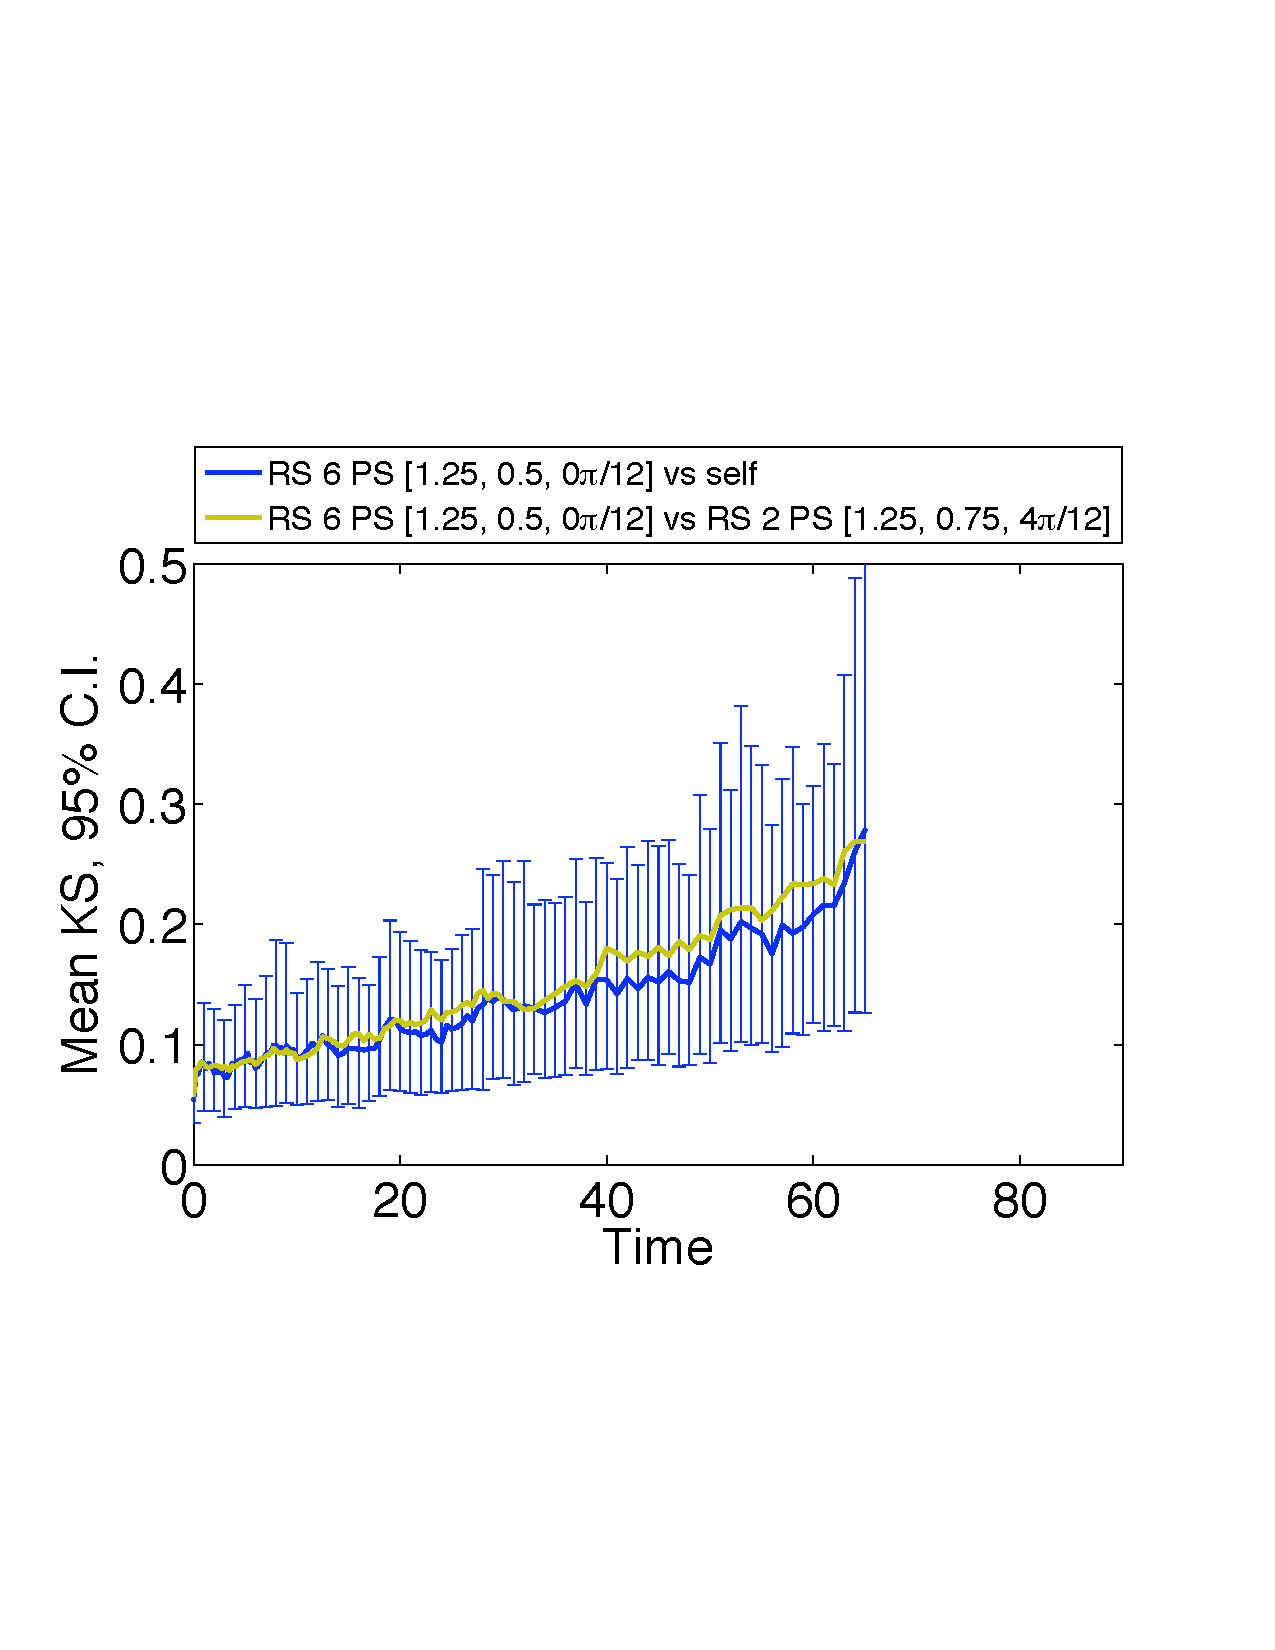
\includegraphics[width=3.25in]{figures/KSstatPerturb_RS06PS012_vs_RS02PS027.pdf}\\
	B & C \\
\end{tabular}
\caption{Rules 1 and 6 are still acceptable matches to rule 2 under perturbed conditions. Panel A uses the empirical distribution generated by rule 2 as the basis for comparison, while panels B and C use the distributions for rule 1 and rule 6 respectively. Notice that the relative goodness of the match depends on which empirical distribution is used for the comparison.}
\label{ksperturb}
\end{figure}



\section{Other comparisons with rule 2}\label{app:rule2matches}

Comparisons of rule 2 to rules 1, 6, and 10 (diffusion), may be seen in Figs.~\ref{fig:diffempdist}.B and \ref{fig:goodmatches}. Using the empirical distributions of rules 3-5 and 7-9, we exhibit the best matches to rule 2 that we could find below. All comparisons except to rules 3 and 4 show substantial dissimilarity. 

\begin{figure}[htp]
\begin{tabular}{cc}
	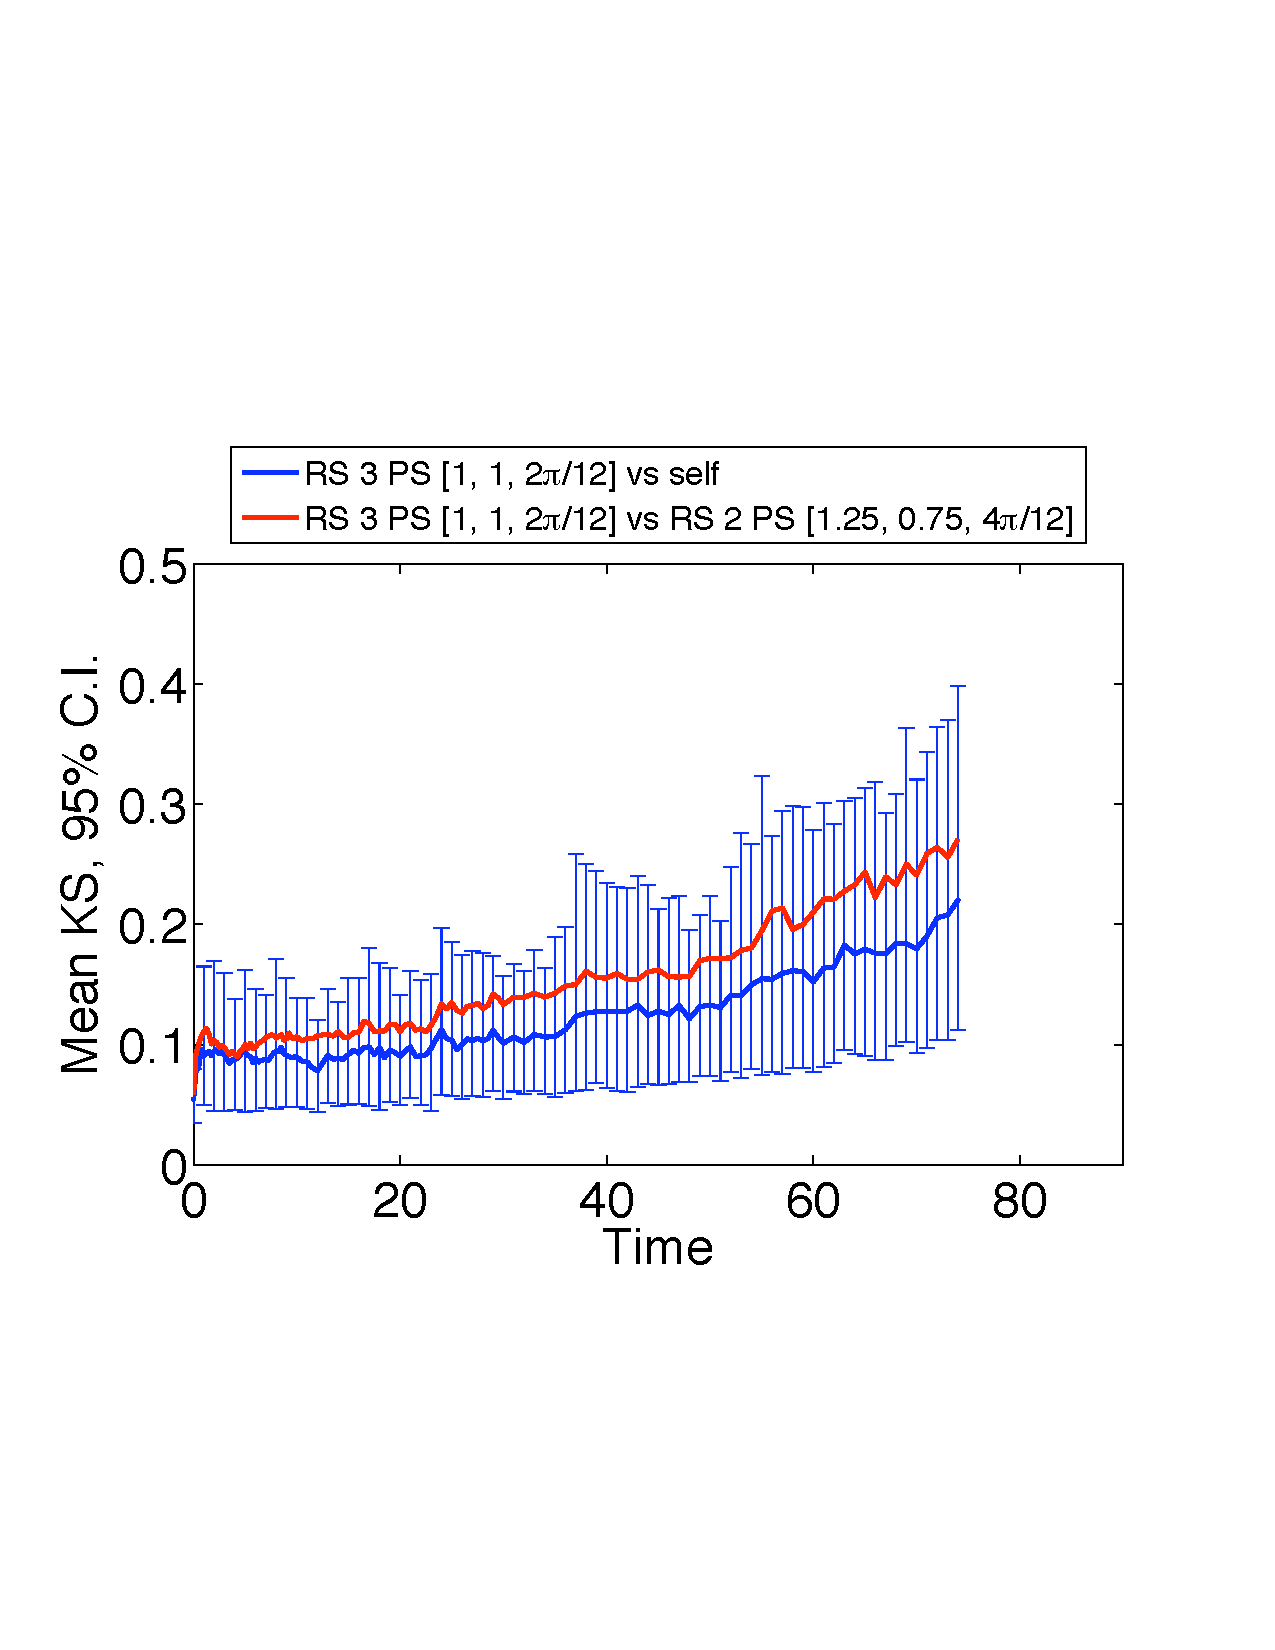
\includegraphics[width=3.25in]{figures/KSstat_RS03PS091_vs_RS02PS027.pdf} & 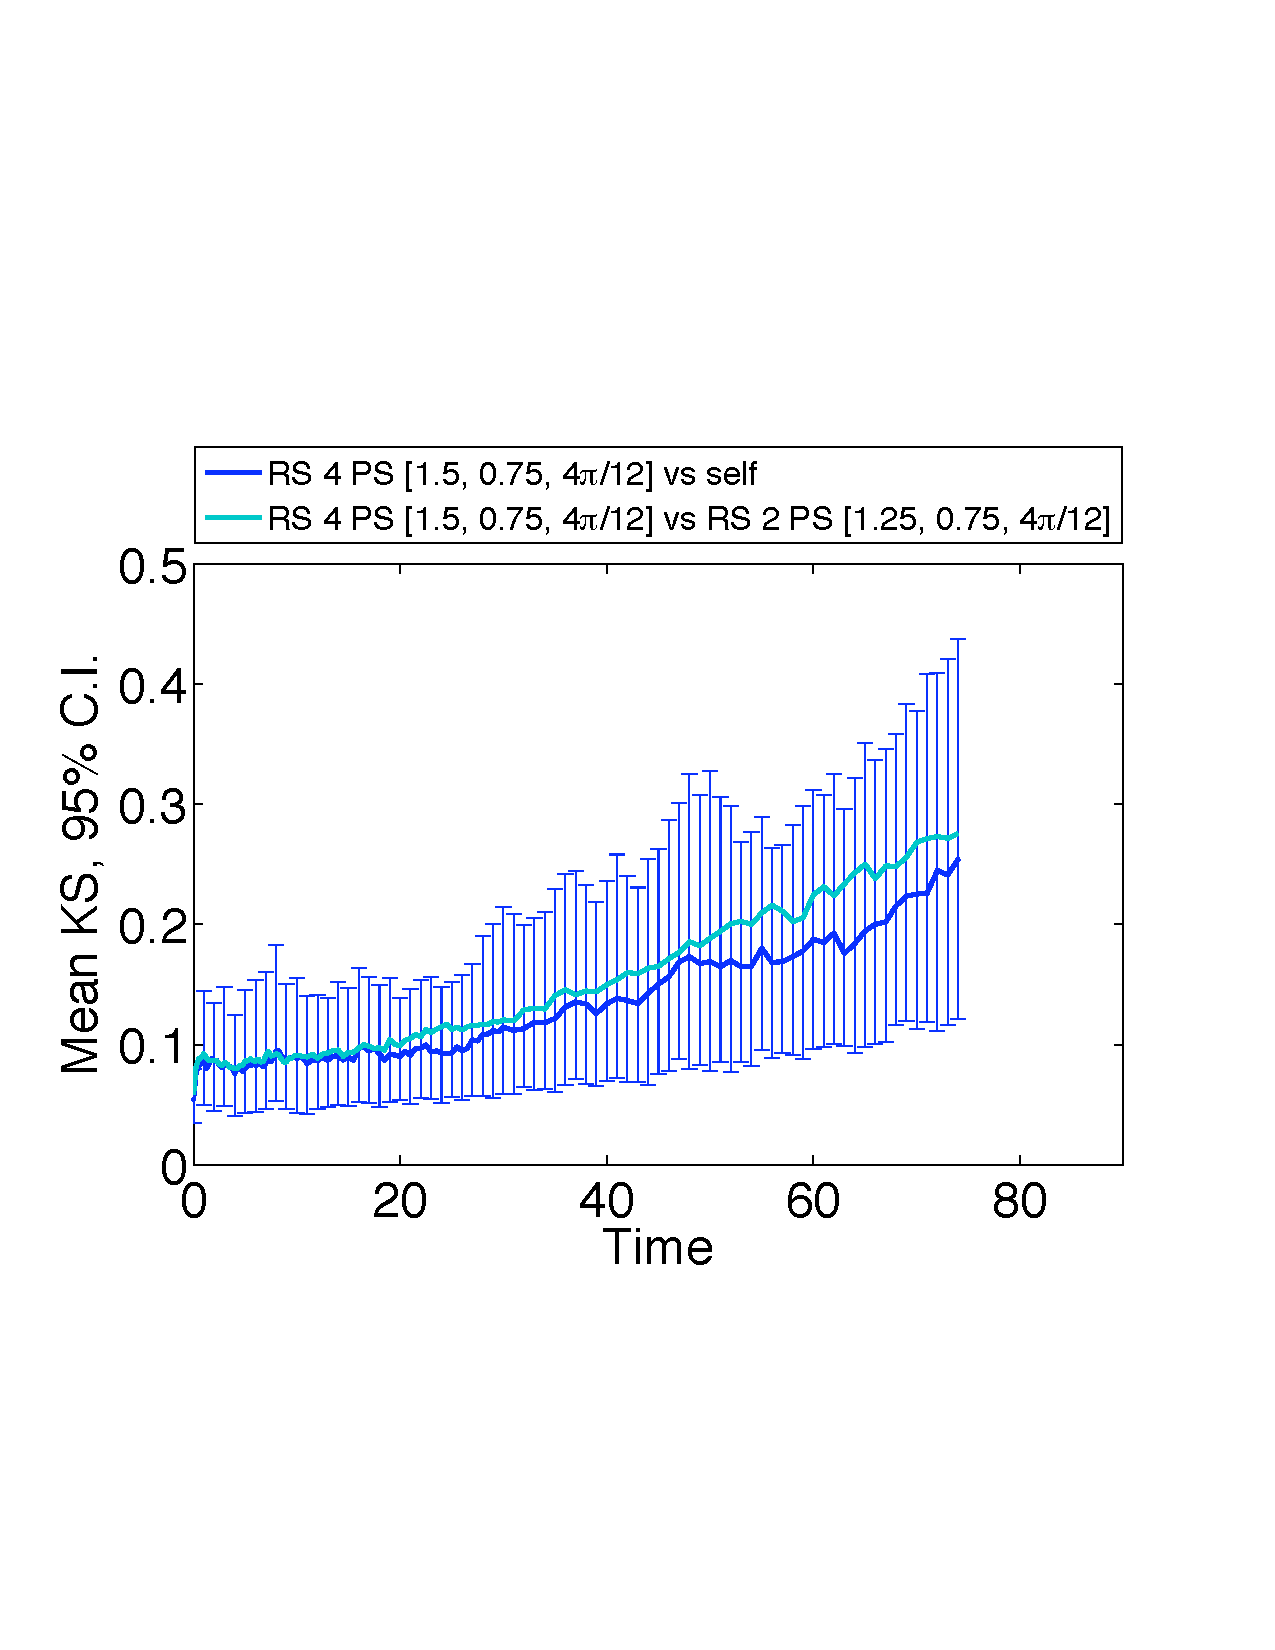
\includegraphics[width=3.25in]{figures/KSstat_RS04PS060_vs_RS02PS027.pdf} \\
	A & B \\
\end{tabular}
\caption{Rules 3 and 4 are tolerable matches to rule 2.}
\label{ksstatsopp3}
\end{figure}

\begin{figure}[htp]
\begin{tabular}{cc}
	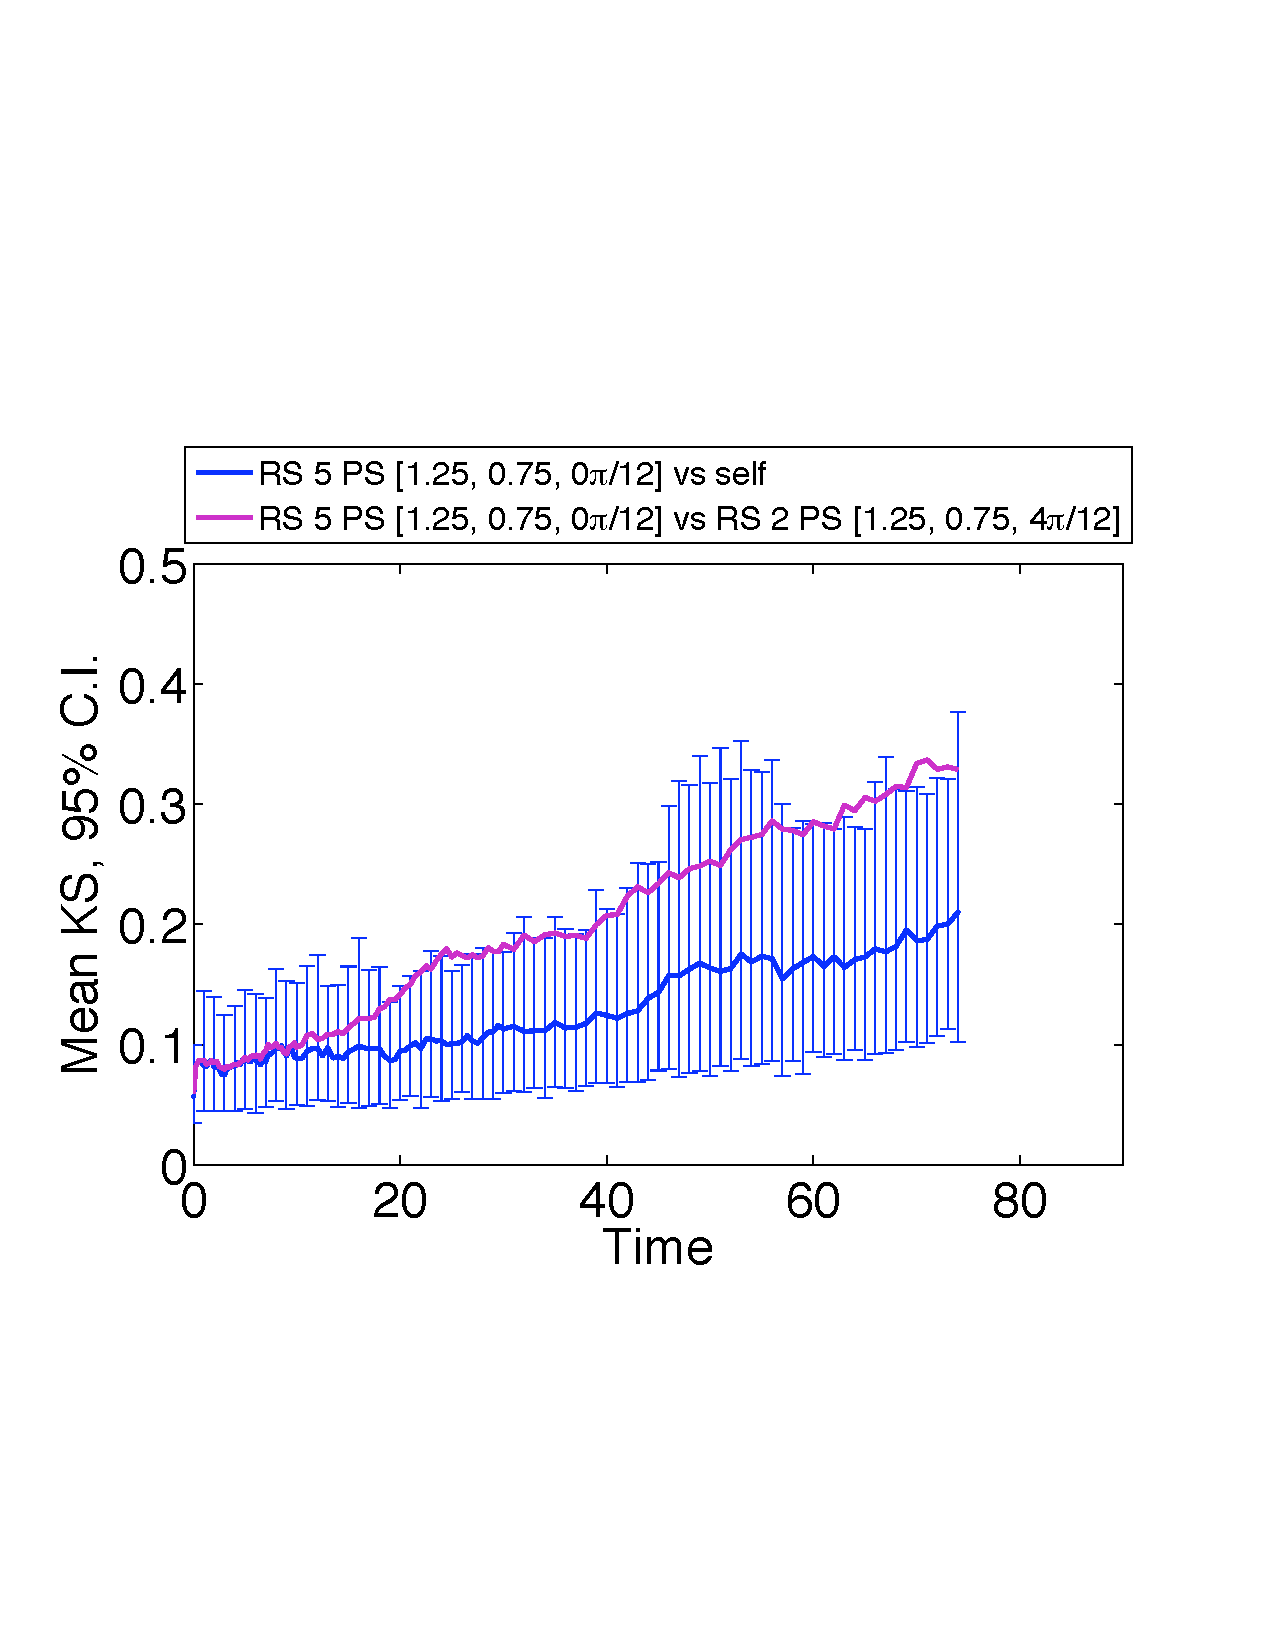
\includegraphics[width=3.25in]{figures/KSstat_RS05PS023_vs_RS02PS027.pdf} & 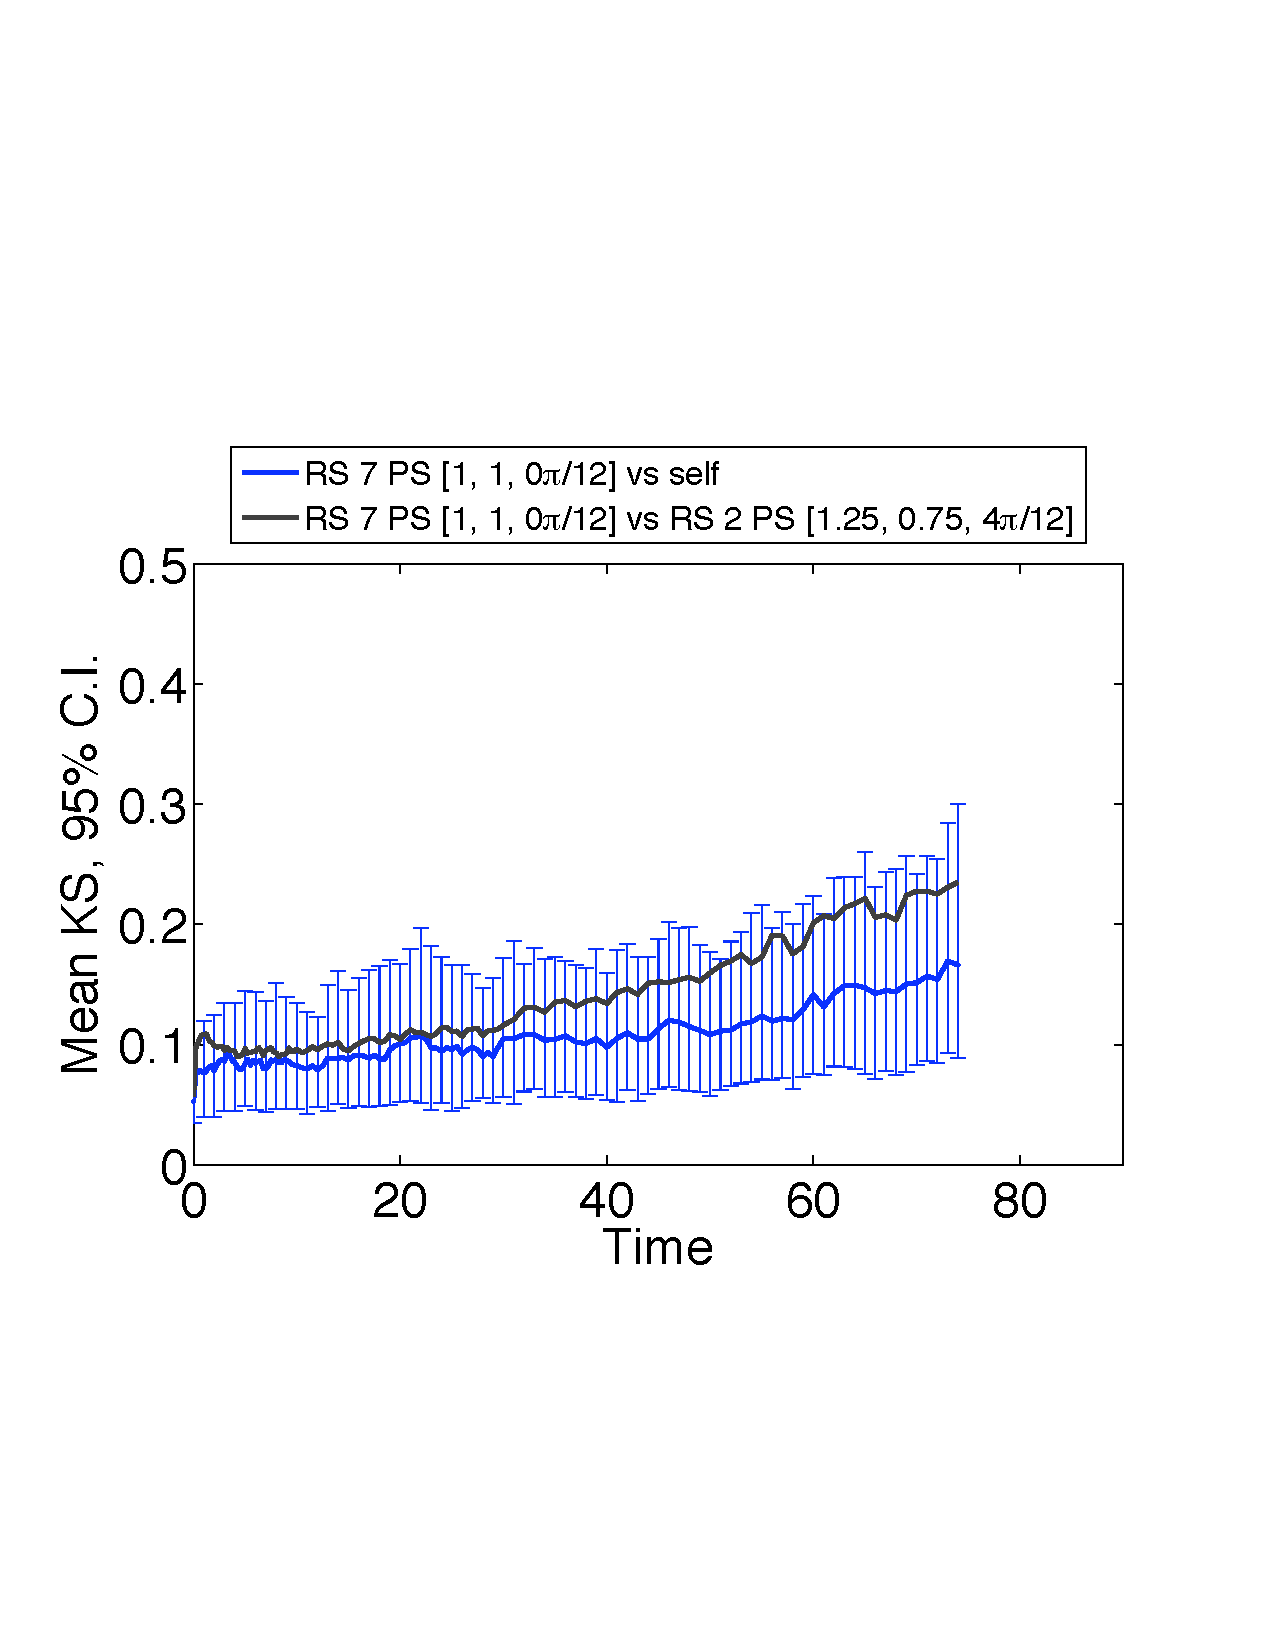
\includegraphics[width=3.25in]{figures/KSstat_RS07PS023_vs_RS02PS027.pdf}\\
	A & B \\
	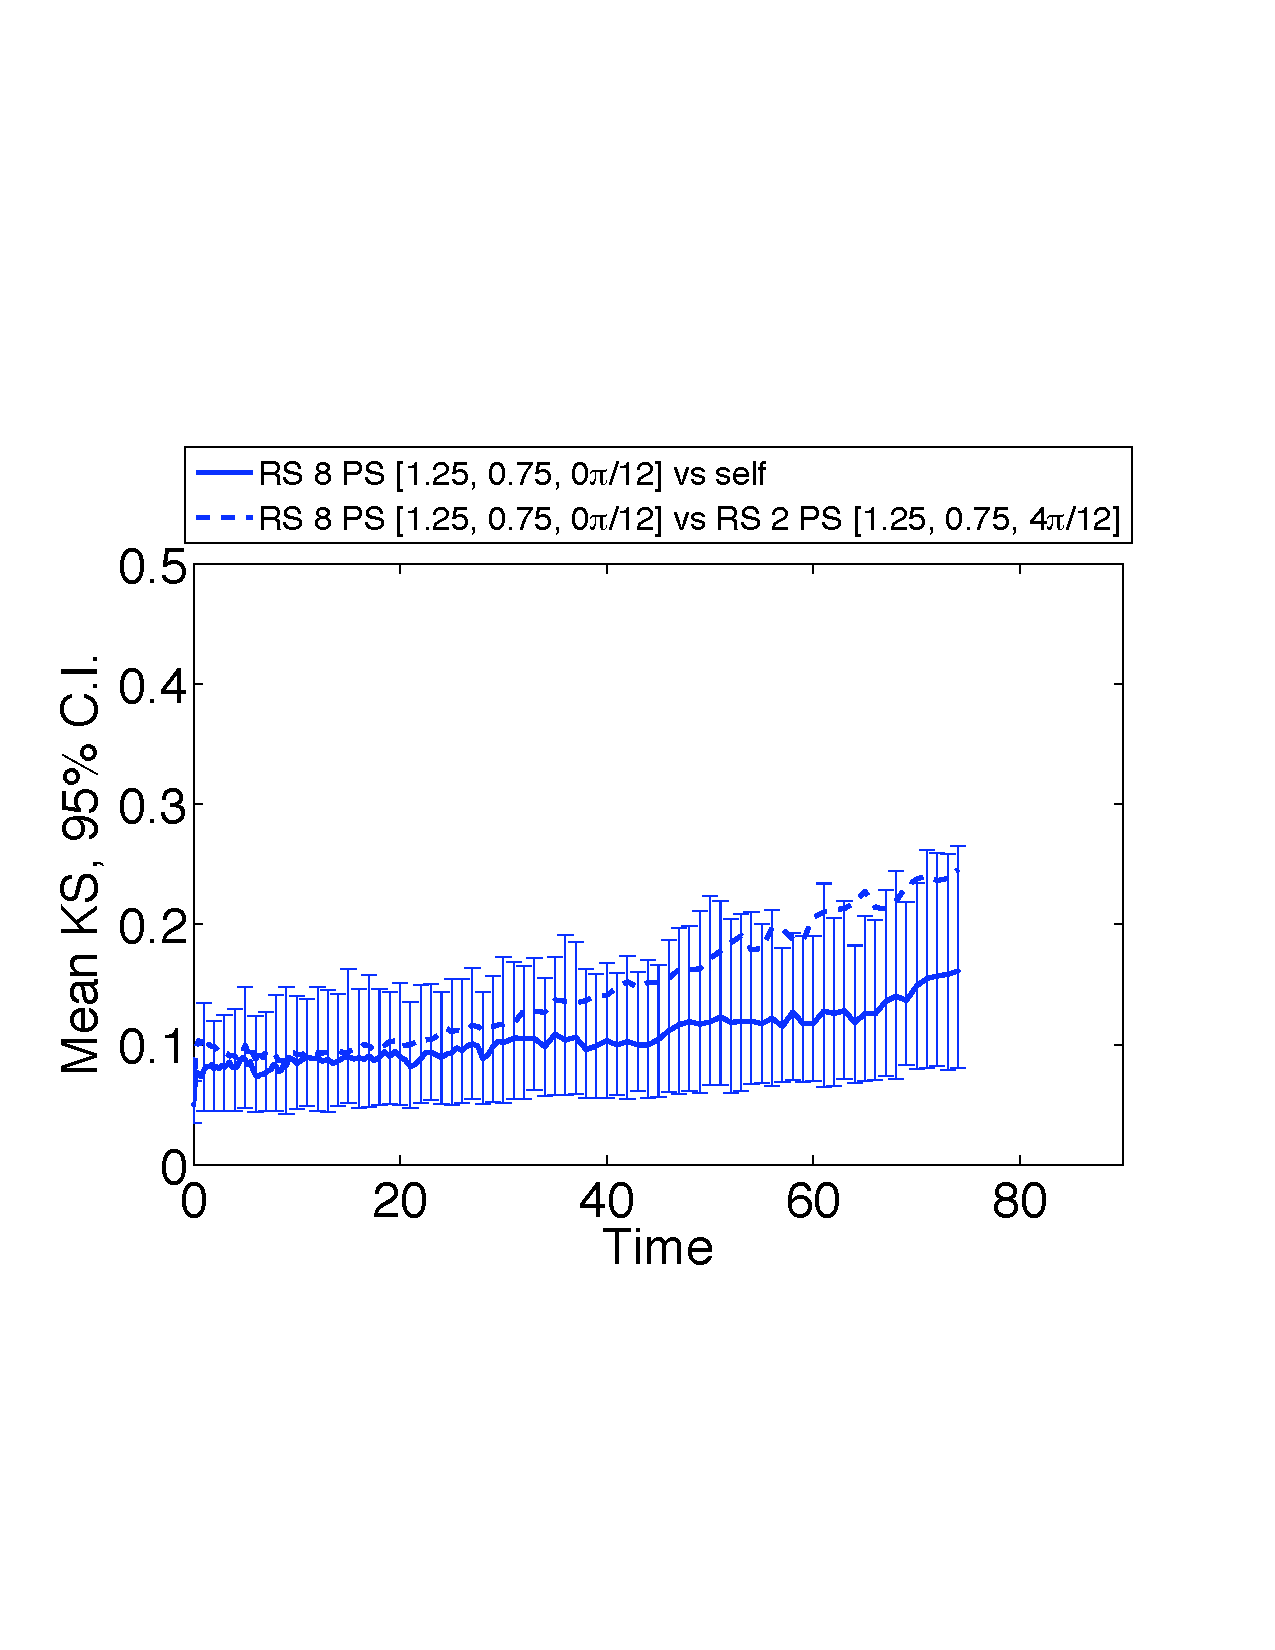
\includegraphics[width=3.25in]{figures/KSstat_RS08PS023_vs_RS02PS027.pdf} & 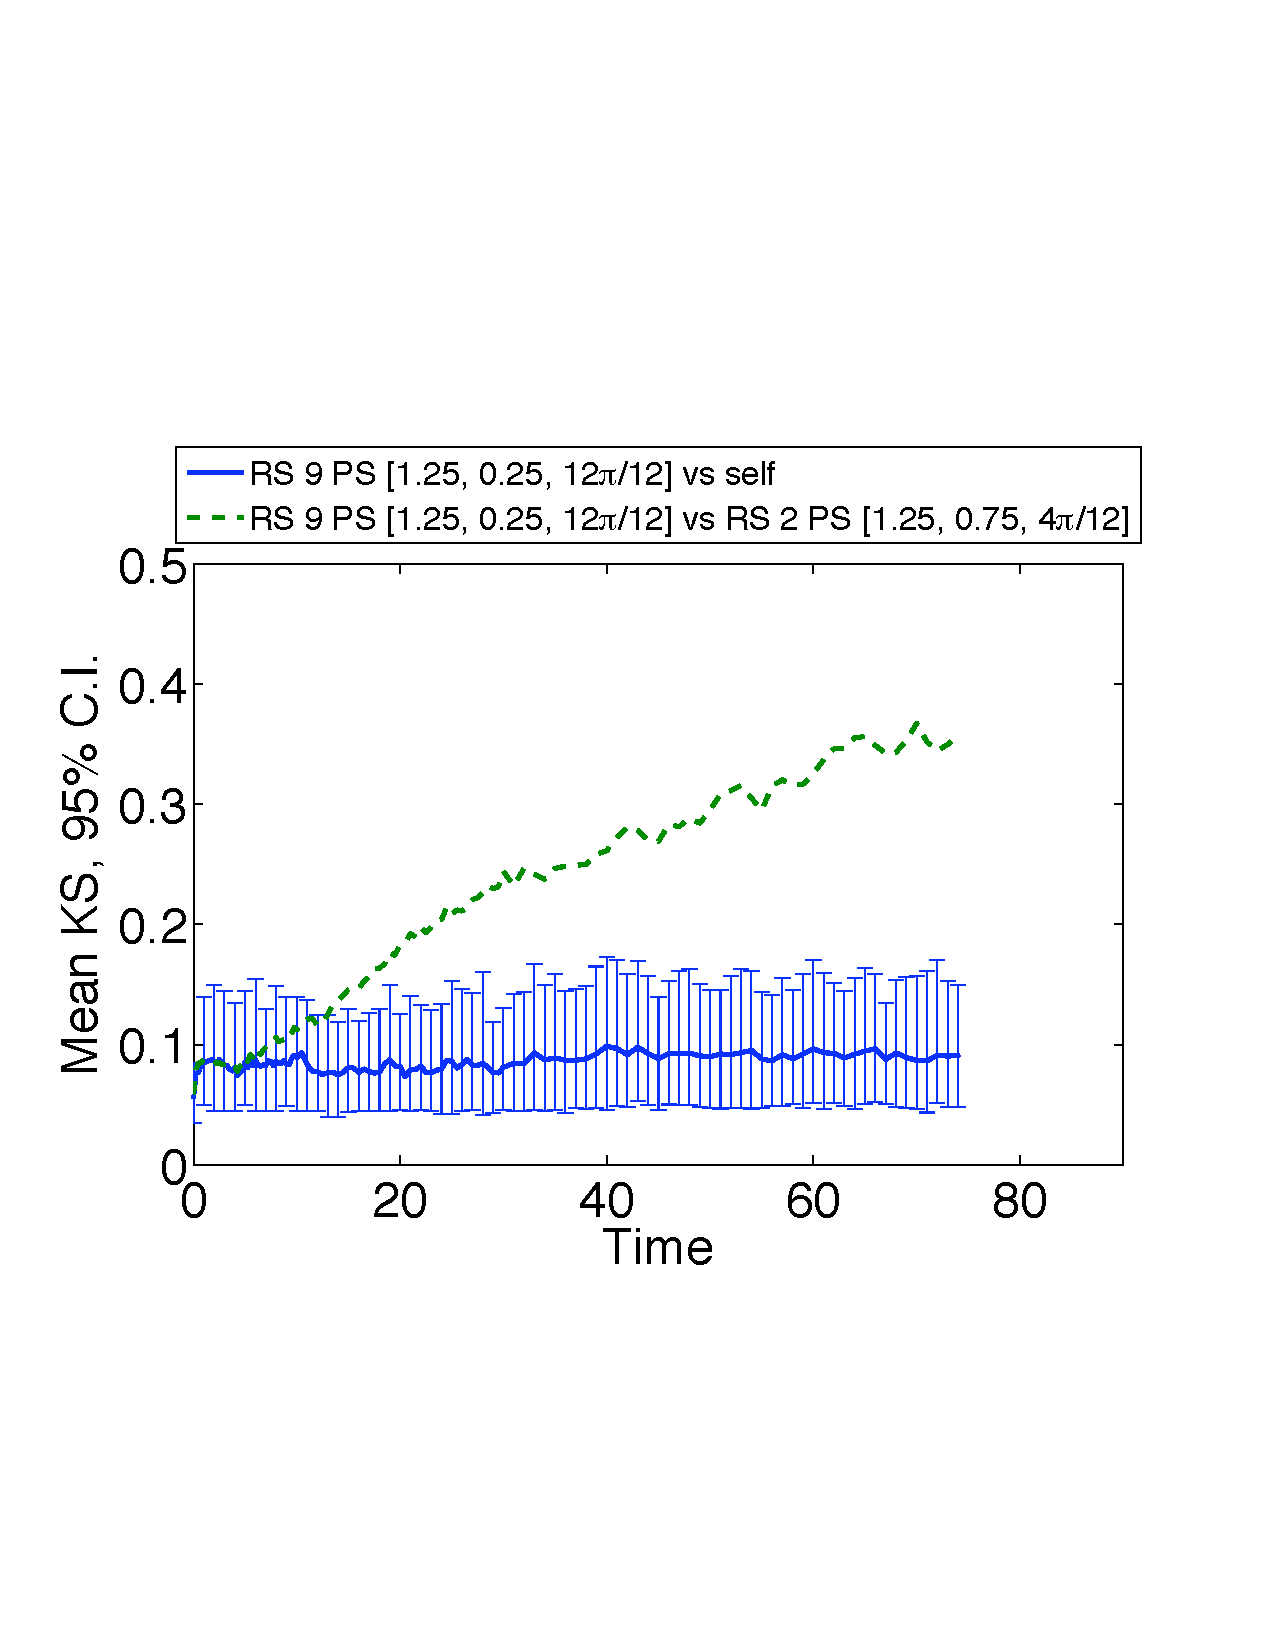
\includegraphics[width=3.25in]{figures/KSstat_RS09PS008_vs_RS02PS027.pdf} \\
	C & D
\end{tabular}
\caption{Rules 5, 7, 8, and 9 are poor matches to rule 2.}
\label{ksstatsopp2}
\end{figure}


\section{Sensitivity to response function concavity}\label{app:kappa}

The response function $F$ in Eq.~\ref{eqn:functional} depends on three parameters: a sensory threshold, $B_0$; a saturation level, $B_{sat}$; and a concavity parameter $\kappa$. We perform some minimal testing of the effect of these parameters on aggregate mosquito behavior using rule 2. In rule 2, we require thresholds and saturation levels for both CO$_2$ concentration ($C$) and for the CO$_2$ gradient ($G$). We fix the parameters $S_1 =  0.75$ m/s, $ S_2 = 1.25$ m/s, $ \beta_1 = \pi/3$, $C_0 = 0.027$ units CO$_2$ per unit air, and $G_0 = 4C_0/L$ units CO$_2$ per unit air per meter ($L$ is the length of one side of the domain). We let $C_{sat}$ vary between two values, 0.8 and 1, and the corresponding $G_{sat}$ is given by $4(C_{sat} - C_0) / L$. We also let $\kappa$ vary between three values, $\kappa_0 = 0$, $\kappa_1 = 200$, and the corresponding negative $\kappa_2$ which is the mirror reflection of $\kappa_1$: $\kappa_2 = -\kappa_1/(1 + \kappa_1 b_0 (1+b_0))$, where $b_0 = B_0/B_{sat}$. This means that there are two different $\kappa_2$, one for the concentration and one for the gradient. 

In total, there are six different parameter sets that we tested. Using the statistical methodology outlined in Section~\ref{sec:chemostats}, we compared all of them to the first parameter set ($\kappa = 0$ and $C_{sat} = 1$), which, except for $C_0 = 0$, is the parameter set for rule 2 that we have been exploring all along. We find only minor differences, and conclude that the model is not overly sensitive to the concavity of the response function (see Fig.~\ref{fig:kappa}). It seems likely to be equally insensitive to other classes of monotonic response functions, e.g. logistic functions. \comment{Bree: For completeness, I should look at the comparisons wrt the empirical distributions generated by the other rule sets. Empirical distributions 3 and 6 are farther from the others.}

\begin{figure}[htp]
\begin{center}
	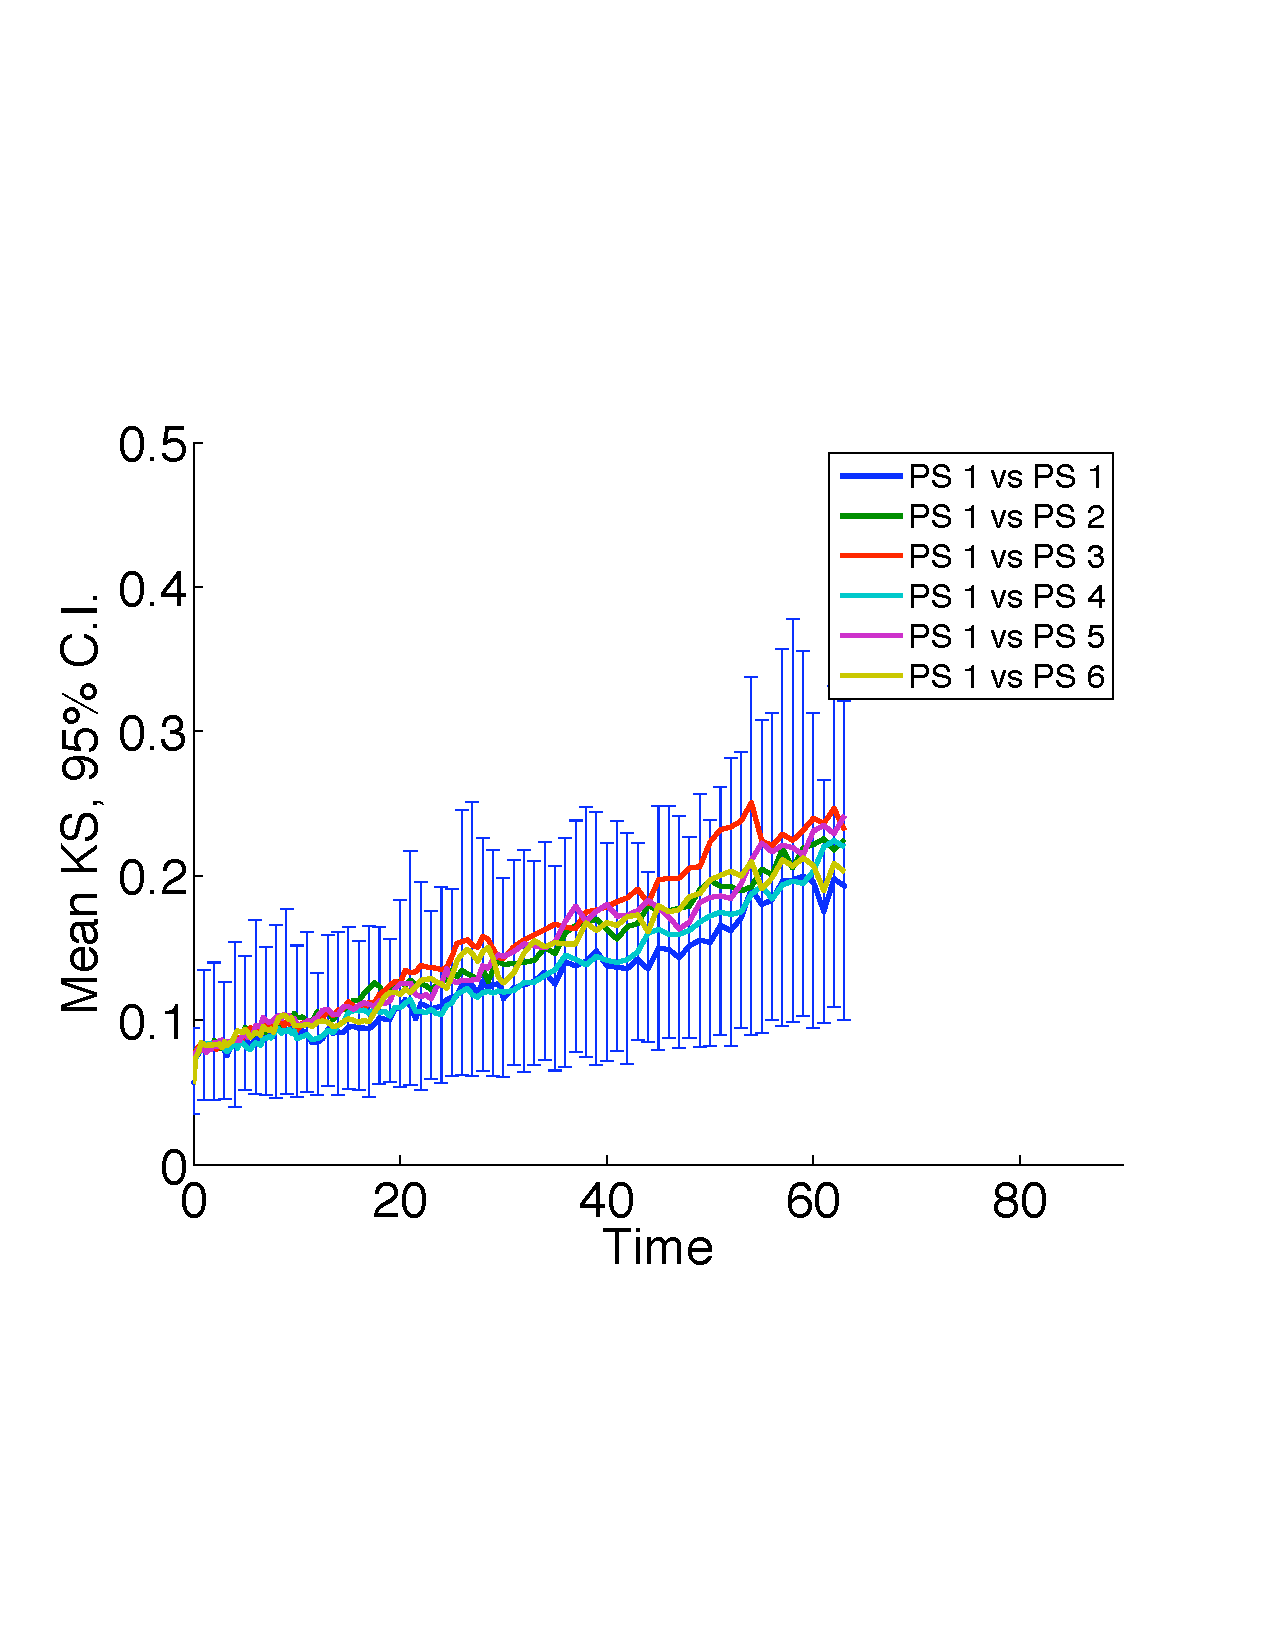
\includegraphics[width=4.0in]{figures/kappacomparisons} 
\end{center}
\caption{Parameter sets (PS) 1 and 4 correspond to $\kappa_0$, 2 and 5 correspond to $\kappa_1$, and 3 and 6 correspond to $\kappa_2$. PS 1-3 have the higher saturation level. The linear functions ($\kappa_0$) are the most similar to each other, but all of the parameter sets are well within the confidence interval, indicating that in general they cannot be distinguished.}
\label{fig:kappa}
\end{figure}





\bibliographystyle{plain}	
\newpage\bibliography{biblio}


\end{document}